% !TEX root = ../../main.tex
% !TEX encoding = UTF-8 Unicode
\chapter{Event Selection}
\label{ch:event_selection}
The event selection is largely based on the strategy and optimizations from the previous Run-II analysis (13.2\,\ifb)~\cite{ichep2016supportnote, lvqq_conf_2016}. Additional optimizations have been made, as described in~\App{\ref{ch:opt}}. Among the improvements is the addition of a VBF signal region, an additional multijet cut, use of the large-R jet combined mass, and a redefinition of the signal regions to utilize both the 50\,\% and 80\,\%  $V$-tagging efficiency working points of the SmoothedWZTagger for the large-R jet identification. 

% How much gain in sensitivity for new LP wp, and VBF category?
% HP+LP fit improves sensitivity by 10\,\%

%
\section{Dataset}
This thesis is based on the full dataset from 2015-2016 $pp$ collisions with center-of-mass energy $\sqrt{s}=13\,\TeV$ recorded by the ATLAS experiment. Only events from ``good'' LBs are used, as defined by the ``Good Run List'' (GRL, \Sect{\ref{ch:event_selection:pre}}), corresponding to a total integrated luminosity of 36.1\,\ifb. A summary of the luminosity and PU conditions is presented in~\Tab{\ref{tab:data_lumi}}.
\begin{table}[htbp]
\centering
\begin{tabular}{c|ccc}
\hline\hline
Year & Max. $\mathcal{L}_{\rm inst.}$ [cm$^{-2}$s$^{-1}$]&$\int\mathcal{L}dt$ [\ifb]&$\langle\mu\rangle$\\\hline
2015&$0.50\times10^{34}$ & 3.2 &3.7 \\
2016&$1.37\times10^{34}$&32.9&24.9\\\hline\hline
\end{tabular}
\caption[Luminosity and pileup conditions of 2015 and 2016 data]{The maximum instantaneous luminosity, total integrated luminosity, and average simultaneous interactions per bunch crossing, $\langle\mu\rangle$, for data recorded by the ATLAS detector in 2015 and 2016. }
\label{tab:data_lumi}
\end{table}

%
\section{Trigger Selection}
This search includes an isolated, high-\pT electron ($e$-channel) or muon ($\mu$-channel) from the leptonic $W$ boson decay; thus, triggering algorithms sensitive to these leptons are used as a first step in reducing the dataset size. The trigger selection is listed in~\Tab{\ref{tab:trig_sel}}. 

\begin{table}[htb]
\centering
\resizebox{\columnwidth}{!}{
\begin{tabular}{l|c|c}
\hline\hline
Data Period&$e$-channel&$\mu$-channel\\\hline
&HLT\_e24\_lhmedium\_L1EM20 OR&\\
2015&HLT\_e60\_lhmedium OR&HLT\_xe70\\
&HLT\_el120\_lhloose&\\\hline
2016a (run $<$ 302919)&HLT\_e26\_lhtight\_nod0\_ivarloose OR&\\
($\mathcal{L}_{\rm inst.}<1.0\times 10^{34}$cm$^{-2}$s$^{-1}$)&HLT\_e60\_lhmedium\_nod0 OR&HLT\_xe90\_mht\_L1XE50\\
&HLT\_el140\_lhloose\_nod0&\\\hline
\vbox{\hbox{\strut 2016b (run $\geq 302919$)}\hbox{($\mathcal{L}_{\rm inst.}<1.4\times 10^{34}$cm$^{-2}$s$^{-1}$)}}&same as 2016a&HLT\_xe110\_mht\_L1XE50\\\hline\hline
\end{tabular}
}
\caption[Summary of lepton triggers used]{Summary of the electron and \MET triggers used in this search.}
\label{tab:trig_sel}
\end{table}

%isolation: $\pT^{\rm cone 20}/\pT<0.10$ for iloose. 
%e60 (non-isolated single e trigger)
For the $e$-channel, the lowest $E_{\rm T}$-threshold, un-prescaled\footnote{
Prescaled triggers randomly reject a fixed fraction of events, in order to keep their output event rate manageable.
}, single-electron triggers are considered. A logical OR between the three triggers is used to select events. The\\ HLT\_e26\_lhtight\_nod0\_ivarloose trigger requires electrons at HLT level with $E_{\rm T} > 26\, \GeV$, tight likelihood-based identification, no transverse impact parameter requirements, and loose variable cone isolation requirements. The higher $E_{\rm T}$ triggers have no isolation requirements, and progressively looser identification requirements. Since the triggering rates scale with the instantaneous luminosity, the lowest $E_{\rm T}$-threshold for un-prescaled triggers was increased in 2016 to maintain manageable event recording rates. The $\pT$-threshold for signal electrons, defined in \Sect{\ref{ch:objreco:el}}, is chosen $1\,\GeV$\, above the trigger threshold to account for offline calibration effects that may lead to different measurements of electron $\pT$ at trigger level and offline reconstruction level. The efficiency of the electron triggers is at least 90\,\% in the plateau region, as shown in~\Fig{\ref{fig:trig_eff}}~\cite{trig_eff_2016}.

\begin{figure}[htbp]
\centering
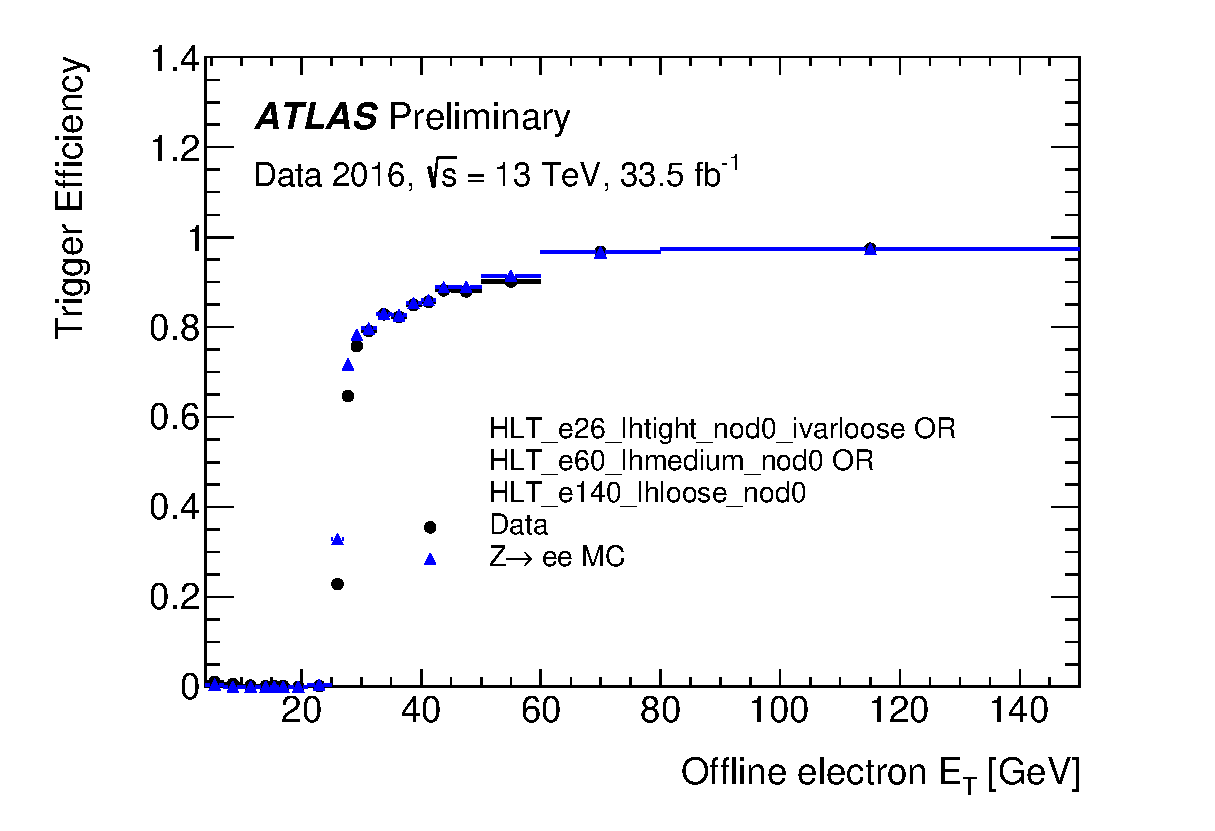
\includegraphics[width=0.55\textwidth]{figures/EventSelection/Eff_Et_singleOR_full2016}
\caption[Electron trigger efficiencies for 2016]{The efficiency of the logical OR between the three un-prescaled electron triggers used in this search~\cite{trig_eff_2016}.}
\label{fig:trig_eff}
\end{figure}

The corresponding lowest $E_{\rm T}$-threshold, un-prescaled, single muon triggers have only a 70\,\% efficiency in the plateau region, due to limited coverage of muon trigger hardware. The $\mu$-channel therefore uses a \MET trigger. At the trigger level, \MET is calculated only using calorimeter energy, ignoring contributions from muons in the MS. Effectively, the \MET measured at trigger level corresponds to the $E_{\rm T}(W\ra\mu\nu)$ measured at reconstruction level.  This trigger has an efficiency of approximately 100\,\% for events with \\$\pT(W\ra\mu\nu)>200\,\GeV$. Contamination from events with multiple muons or no muons can be mitigated by requiring exactly one signal muon. The increased acceptance of the \MET trigger corresponds to a 10\,\% improvement in sensitivity in the combined $e+\mu$ channel. Notably, the gain in efficiency is important in the high mass region, which is particularly sensitive to signal acceptance. 

Since \MET is strongly affected by $\langle\mu\rangle$, the \MET trigger thresholds were raised multiple times to combat the rising trigger rates. In 2015, \MET was calculated using the cell method: \MET is calculated as the negative sum of the $E_{\rm T}$ in all calorimeter cells. Starting in 2016, \MET was calculated using the the missing $H_{\rm T}$ (MHT) algorithm. For MHT, the negative vector sum of the \pT of calibrated anti-$k_{\rm T}$ jets is used to define \MET.

%
\section{Event Preselection}
\label{ch:event_selection:pre}
Before the analysis selection cuts are applied, a preselection is imposed to reject events with detector or reconstruction problems, and to reduce the dataset size. The first stage is called event cleaning, and is standardized for ATLAS physics analyses.

\begin{itemize}
\item\underline{Good Runs List}: A GRL selection is applied to ensure the data corresponds to periods of time (lumi-blocks) where the detector was fully operational, and the data collected was of adequate quality. The LHC beams are required to be stable, the magnets are required to be on (and not ramping), and all subdetectors are required to be on, with not too many noisy cells.
\item\underline{Primary Vertex}: The event is required to have a primary vertex with at least two tracks, each with $p_{\rm T, trk}>400\,\MeV$. If more than one vertex satisfies the requirement, the one with the largest $\sum p_{\rm T, trk}^2$ is selected. 
\item\underline{Subdetector Error Veto}: Corrupted events from the LAr and Tile calorimeters, and the SCT are vetoed. Events are also rejected if they occur close to a noise burst in the LAr calorimeter. 
\item\underline{Incomplete Events}: If for any reason a recorded event is missing detector information, it is rejected.
\end{itemize}

After the event cleaning cuts, the rest of the preselection cuts are applied, where signal and veto leptons are defined in~\Ch{\ref{ch:objreco}}:

\begin{itemize}
	\item\underline{Bad Jet Veto}: Noise bursts or coherent noise in the calorimeters, hardware issues, beam backgrounds, and cosmic muons can create fake jets. A high efficiency working point, called BadLoose, is defined to reject events with ``bad" jets~\cite{bad_jet}. These bad jets can degrade the calculation of \MET. Since electrons and muons can be reconstructed as bad jets, the overlap removal procedure between signal and veto leptons and jets is applied before the bad jet veto.  %\href{https://twiki.cern.ch/twiki/bin/view/AtlasProtected/HowToCleanJets2016}{Veto whole event} if there is a badjet after overlap removal.
    \item\underline{Second Lepton Veto}: The event is required to have exactly one lepton, with no ``veto'' leptons.
 	\item\underline{Signal lepton}: The lepton is required to pass the signal lepton definition.
	\item\underline{Trigger Matching}: The reconstructed signal lepton is required to match the physics object that passed the initial trigger. 
	%\item {$\pt(\ell\nu) > 75\,\GeV$}
	%\item {At least one large-R jet}
\end{itemize}

%
\section{Event Reweighting}
The generated MC samples require various weights in order to ensure their distribution agrees with the distribution observed in data. As mentioned in~\Sect{\ref{ch:analysisStrategy:sig_bkg_model}}, a PU reweighting is applied to MC samples to match the measured PU distribution. Weights are also applied due to the different efficiencies of reconstructed objects from MC and from data. For leptons, weights are applied to correct for reconstruction and isolation efficiencies. Electrons have additional weights for identification, and for trigger and matching efficiencies. Muons have weights applied for the efficiency of associating tracks to a vertex. Jets have weights applied due to efficiencies of $b$-tagging~\cite{b_jet} and the jet vertex tagger. Finally, the MC samples are scaled to the measured integrated luminosity, taking into account higher order corrections to cross sections and filter efficiencies (enforcing a specific final state, e.g. leptonic decay of a top quark).
%$N_{exp} = \sigma \times BR \times \mathcal\times k_{factor}\times \epsilon_{filter}\times{L}_{int}$
% $N_{pred} = N_{gen, pass selection} \times N_{exp} / N_{generated}$

%
\section{Event Categorization by Production Mechanism}
After preselection, events are categorized according to whether they are compatible with VBF production. As motivated in~\Sect{\ref{ch:evt_sel:sig_eff}}, the VBF production region is prioritized.  Events passing the selection criteria are categorized as ``VBF selection'', while, for brevity, events failing the selection criteria are categorized as ``ggF selection'', where the ggF selection is meant to encompass qqF production as well. 
%Moreover, there can be signal leak between categories, but every event will be classified as either a VBF selection or ggF selection.

The VBF selection is summarized in~\Tab{\ref{tab:vbf_sel}}. The selection requires at least two VBF candidate small-R jets, as defined in~\Sect{\ref{ch:objectReconstruction:smallr}}. If there are more than two such jets, the two with the highest invariant mass, $m^{\rm VBF}(j,j)$, are selected. Jets from VBF production are expected to have a small deflection from the beamline, thus, the jets are required to be in different hemispheres of the detector, $\eta(j_1)\cdot\eta(j_2)<0$.  The pair of jets are then required to satisfy, $m^{\rm VBF}(j,j)>770\,\GeV$, and have a separation of $|\Delta\eta^{\rm VBF}(j,j)|>4.7$.  

All events that fail the VBF selection are treated in the ggF selection category. The selection efficiency of VBF jets from signal samples with VBF production is approximately 28\,\%. Only 1\,\% of signal samples produced with ggF (or qqF) pass the VBF selection.
% The mass and separation cuts were chosen to harmonize with $llqq$ channel, and is consistent with the maximum sensitivity region of this analysis.

\begin{table}[htb]
\centering
\begin{tabular}{l|c}
\hline\hline
Selection & Requirement\\\hline
Num. VBF candidate jets &$\geq 2$\\
&(if $>2$, select highest $m^{\rm VBF}(j,j)$ pair)\\
Separate Hemispheres&$\eta(j_1)\cdot \eta(j_2)<0$\\
Invariant Mass [\GeV]&$m^{\rm VBF}(j,j)>770$\\
Separation&$|\Delta\eta^{\rm VBF}(j,j)|>4.7$\\\hline\hline
\end{tabular}
\caption[Vector boson fusion event selection criteria]{Summary of the criteria for the VBF event selection.}
\label{tab:vbf_sel}
\end{table}

%
\section{Kinematic and Topological Selections}
After the event is categorized according to the production mechanism, a series of kinematic and topological cuts are placed in order to select events from the boosted regime. 
\begin{itemize}
\item\underline{Large-R Jet}: At least one large-R jet satisfying the definition in~\Sect{\ref{ch:objectReconstruction:larger}} is required. If more than one exists, the one with the largest $\pT$ is selected. For the VBF event selection, the large-R jet is required to not overlap with the VBF selected jets: $\Delta R(j_1^{\rm VBF},J)>1.5$ and $\Delta R(j_2^{\rm VBF},J)>1.5$.
\item\underline{Multijet Cleaning:} Requiring $\MET>100\,\GeV$\, removes nearly all the multijet background. A further requirement is placed to remove a small number of multijet events which fake a high-\pT electron with an associated low amount of \MET. The $e$-channel is required to satisfy: $\MET/\pT(W\ra e\nu)>0.2$. The multijet background is estimated to be negligible after these cuts, as detailed in~\App{\ref{ch:qcd}}. 
\item\underline{Boosted Regime:} The leptonically decaying boson is required to be sufficiently boosted: $\pT(W\ra\ell\nu)>200\,\GeV$. This also ensures the \MET trigger is fully efficient in the $\mu$-channel.
\item\underline{Relative Boson \pT}: Since the weak bosons from the resonance decay are expected to have \pT equal to approximately half the resonance mass, events are rejected if the ratio of the weak boson \pT to the invariant mass of the $WV\ra\ell\nu J$ system is too low. The optimal cut values were found not to depend on signal mass, and for simplicity, the thresholds for the leptonic and hadronic decays are equal. The VBF threshold is lower to increase signal efficiency. 
\begin{itemize}
\item $\pT(W\ra\ell\nu)/m(WV\ra\ell\nu J) > 0.3\, (0.4)$ for VBF (ggF) selection
\item $\pT(J)/m(WV\ra\ell\nu J) > 0.3\, (0.4)$ for VBF (ggF) selection
\end{itemize}
\end{itemize}



%
\section{Signal and Control Regions}
\label{ch:eventSelection:srcr}
This search is sensitive to both charged and neutral resonances. Two channels exist, corresponding to whether the large-R jet is tagged as a $W$ or $Z$ boson. Since the SmoothedWZTagger uses a mass window to identify the boson, there is a large overlap between the $WW$-channel and the $WZ$-channel. The overlap is acceptable since signal models will only be evaluated in one channel. Both the 50\,\% and 80\,\% efficiency working points of the SmoothedWZTagger are used to define the signal regions (SR) and control regions (CR). A high purity (HP) region is defined in~\Sect{\ref{ch:evt_sel:hp}}, and a low purity (LP) region, meant to recover additional signal events, is defined in~\Sect{\ref{ch:evt_sel:lp}}.

%
\subsection{High Purity Selection}
\label{ch:evt_sel:hp}
The HP selection is designed to have the highest sensitivity to signals in the high mass region, where the SM background is expected to be low. The HP SR is defined by the following selection:
\begin{itemize}
\item\underline{$b$-jet Veto}: Events with a small-R jet tagged as a $b$-jet (\Sect{\ref{ch:objectReconstruction:smallr}}) are vetoed if the $b$-jet lies outside the large-R jet: $\Delta R(J,b)>1.0$. This cut rejects approximately 70\,\% of \ttbar events, while maintaining a signal efficiency of approximately 95\,\%.
\item\underline{Boson Tagging}: The large-R jet is required to pass the 50\,\% efficiency working point for the $W$ or $Z$ boson mass window cut (it is possible for a large-R jet to pass both). Additionally, the large-R jet is required to pass the 50\,\% efficiency working point for the \pT-dependent upper cut on the $D_2^{\beta=1}$ substructure variable. 
\end{itemize}
In~\Fig{\ref{fig:evt_sigbkg_hp}}, shape differences between background and signal MC distributions of the large-R jet mass, $D_2^{\beta=1}$, and relative \pT are shown in the HP SR.

\begin{figure}[tbp]
\centering
\subfloat[]{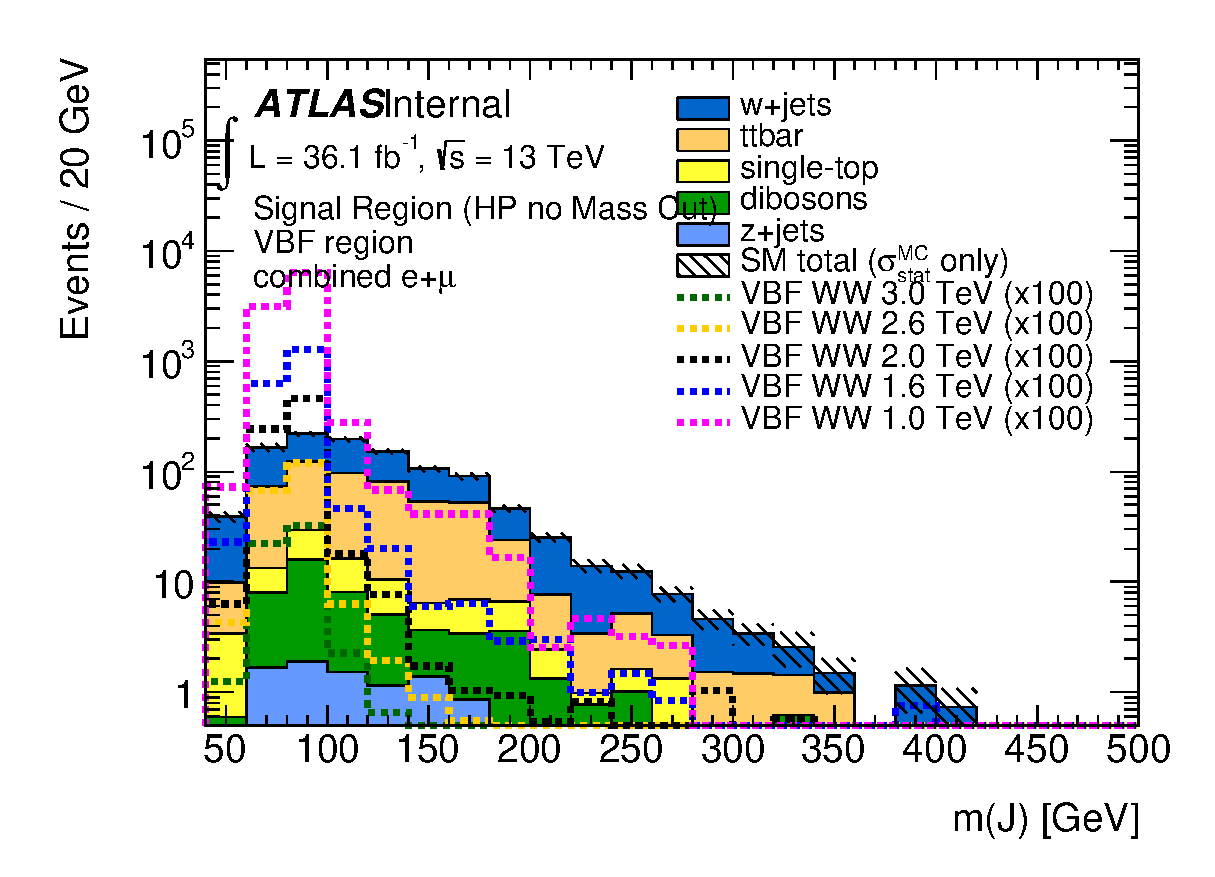
\includegraphics[width=.49\textwidth]{figures/EventSelection/JM_5_comb_VBF}\label{fig:evt_sigbkg_hp:a}}
\subfloat[]{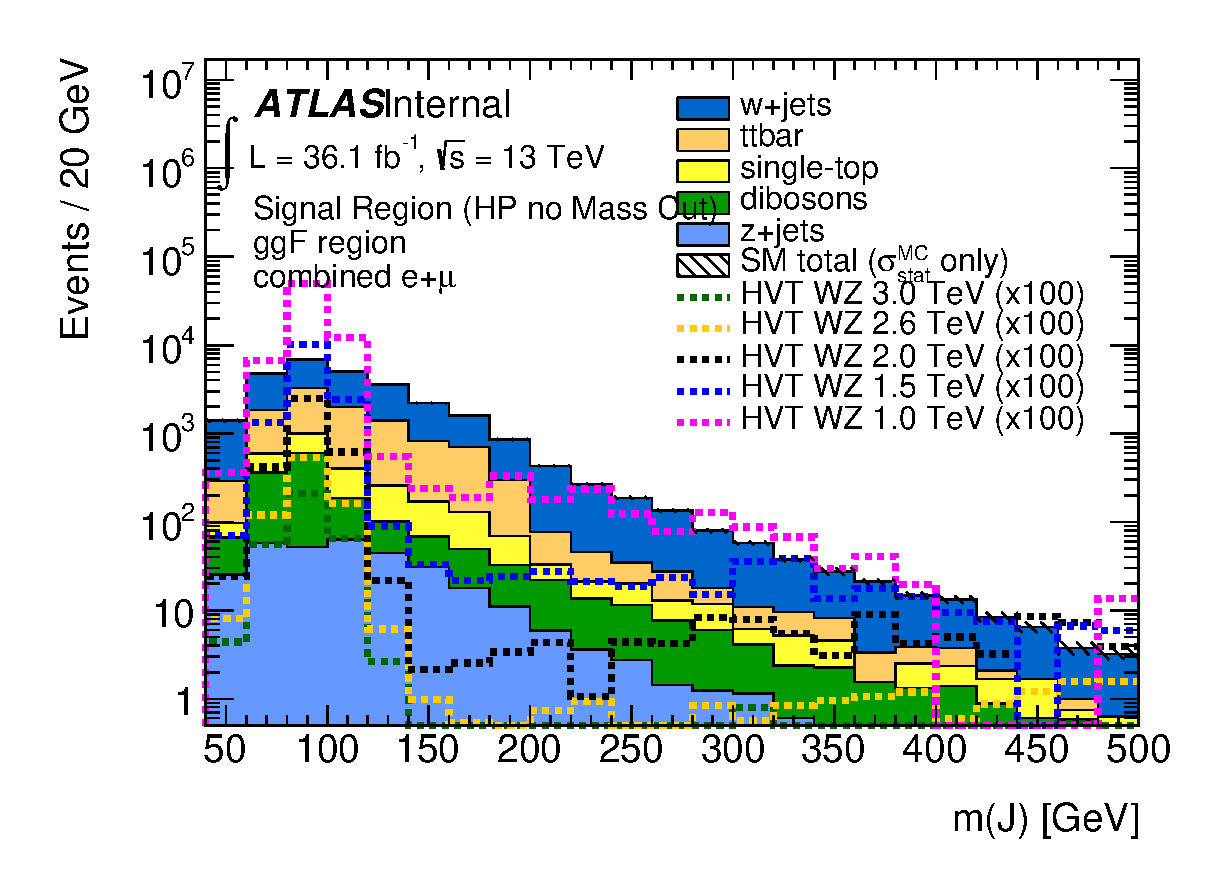
\includegraphics[width=.49\textwidth]{figures/EventSelection/JM_5_comb_ggF}\label{fig:evt_sigbkg_hp:b}}\\
\subfloat[]{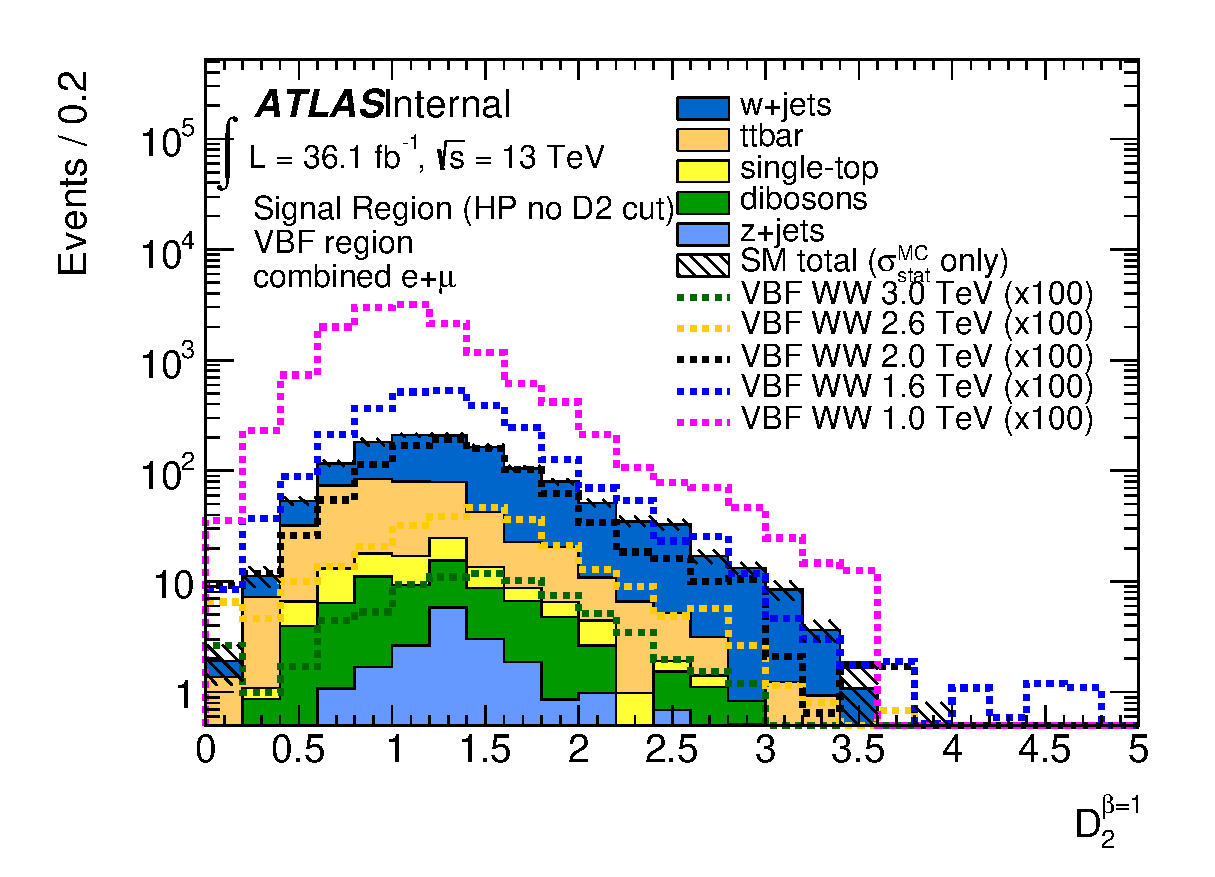
\includegraphics[width=.49\textwidth]{figures/EventSelection/JD2_1_comb_VBF}\label{fig:evt_sigbkg_hp:c}}
\subfloat[]{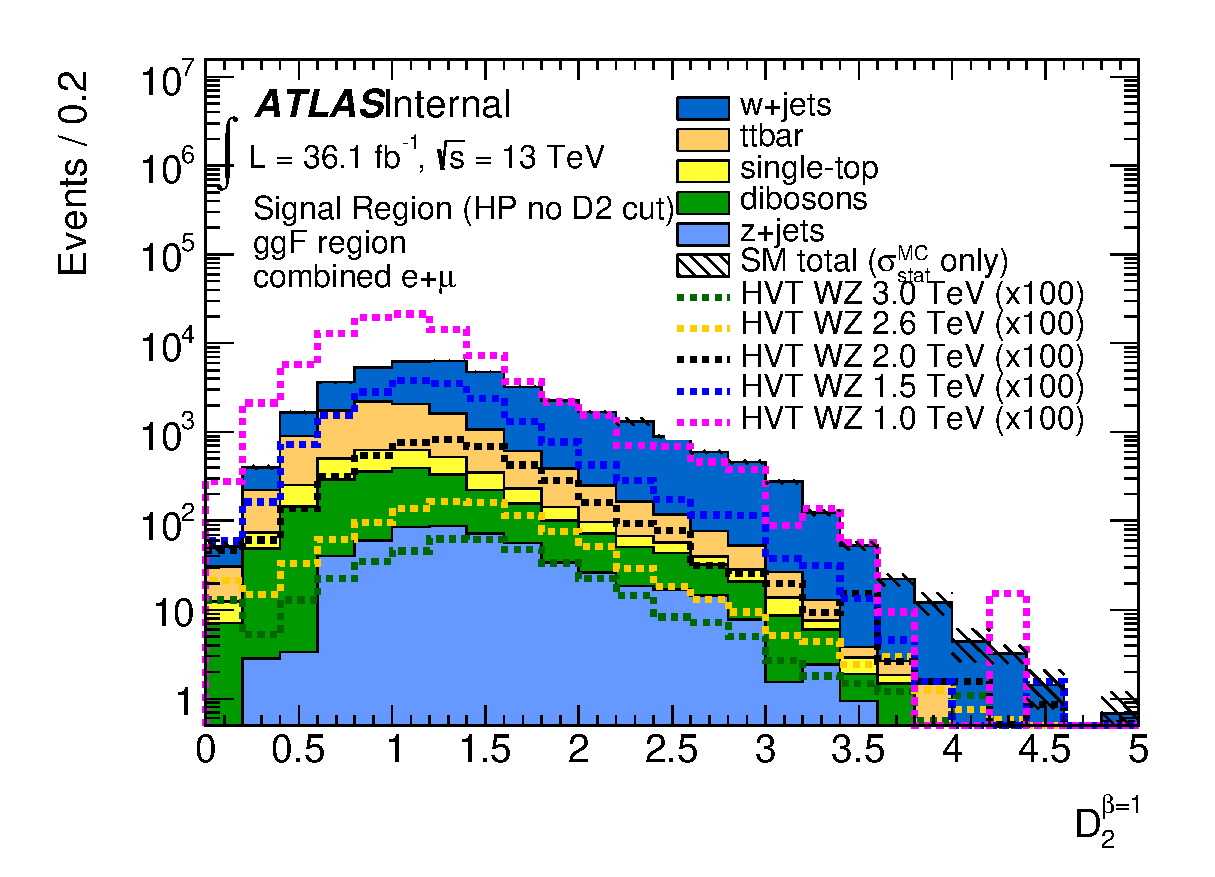
\includegraphics[width=.49\textwidth]{figures/EventSelection/JD2_1_comb_ggF}\label{fig:evt_sigbkg_hp:d}}\\
\subfloat[]{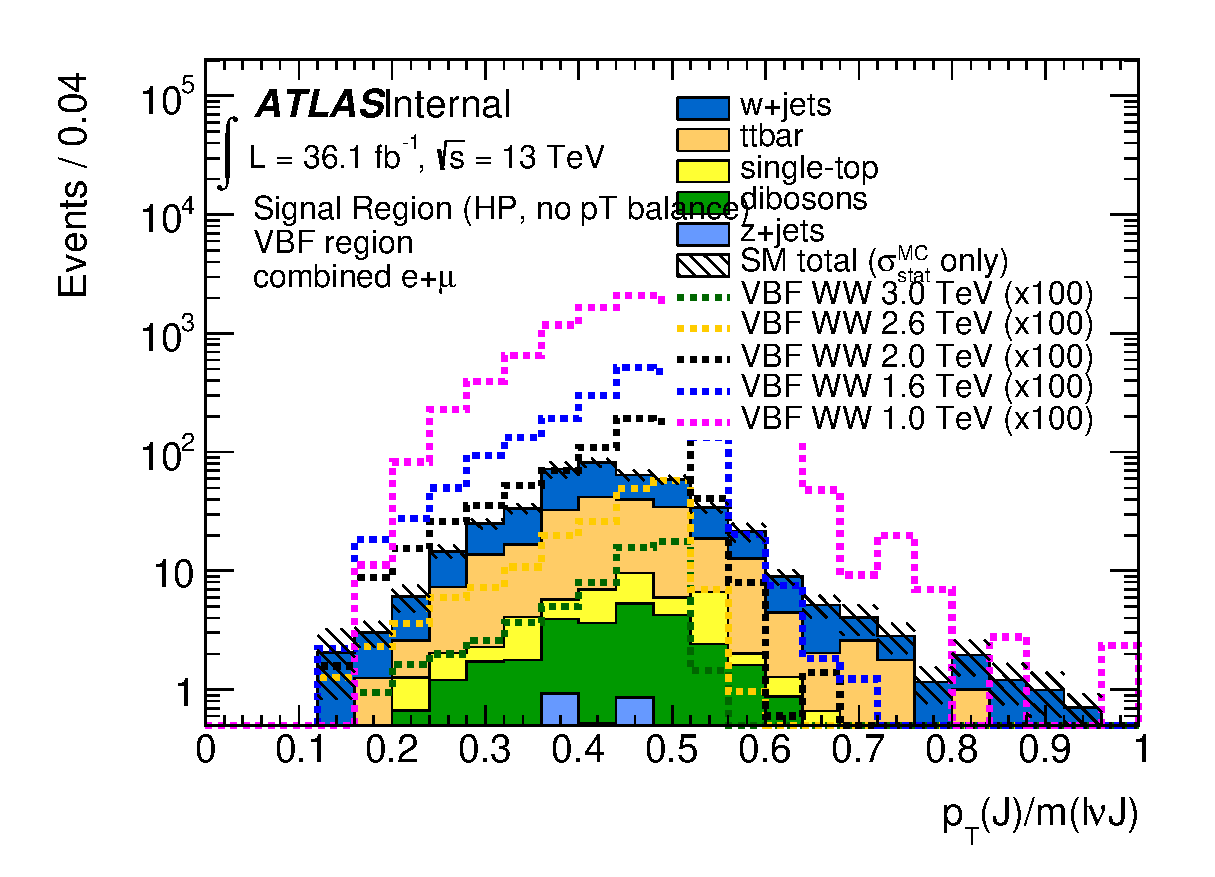
\includegraphics[width=.49\textwidth]{figures/EventSelection/JPt_over_M_6_comb_VBF}\label{fig:evt_sigbkg_hp:e}}
\subfloat[]{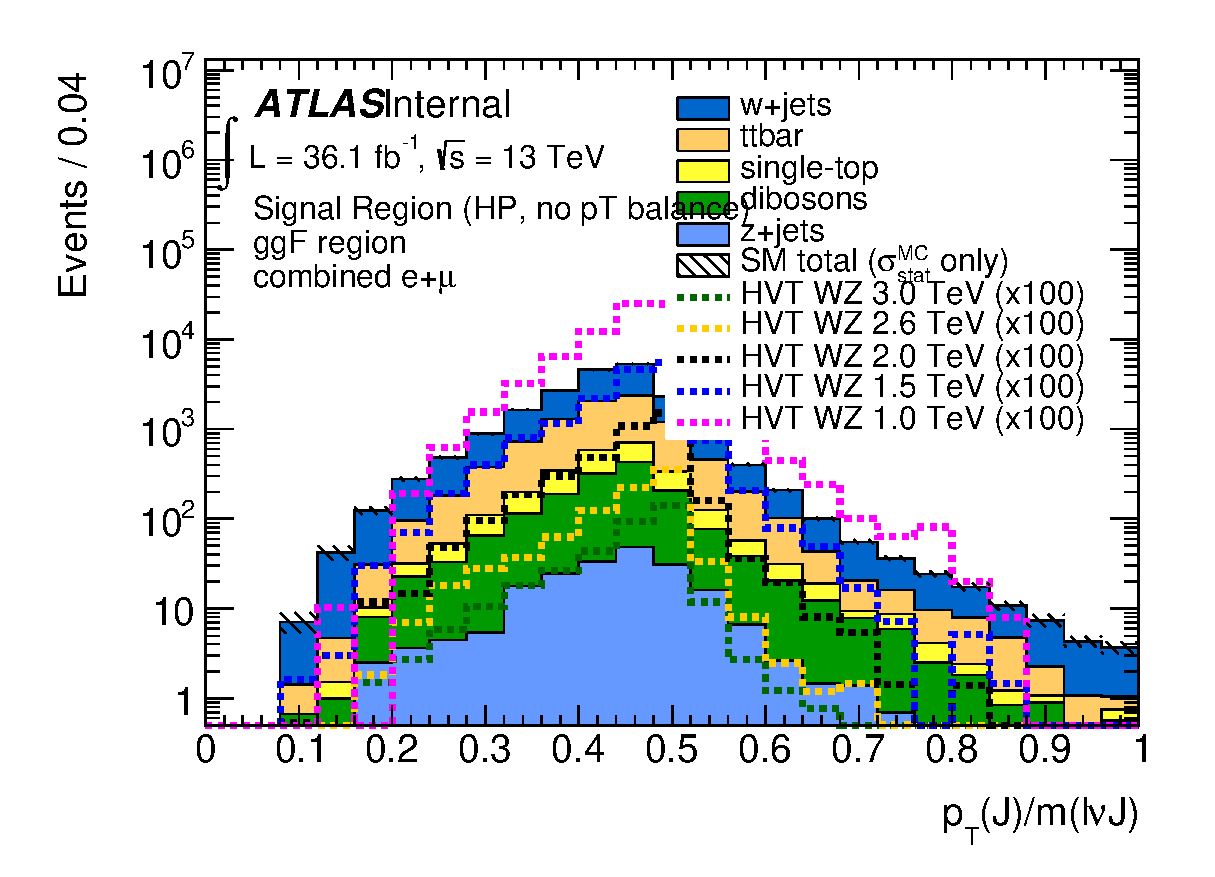
\includegraphics[width=.49\textwidth]{figures/EventSelection/JPt_over_M_6_comb_ggF}\label{fig:evt_sigbkg_hp:f}}
\caption[Large-R jet distributions in the high purity signal regions]{Large-R jet mass in the HP SR (without $m(J)$ window cut) for the \protect\subref{fig:evt_sigbkg_hp:a} VBF and \protect\subref{fig:evt_sigbkg_hp:b} ggF selection. Large-R jet $D_2^{\beta=1}$ distribution in the HP SR (without $D_2^{\beta=1}$ upper cut) for the  \protect\subref{fig:evt_sigbkg_hp:c} VBF and \protect\subref{fig:evt_sigbkg_hp:d} ggF selection. Large-R jet relative \pT in the HP SR (without relative \pT cuts) for the \protect\subref{fig:evt_sigbkg_hp:e}VBF selection and \protect\subref{fig:evt_sigbkg_hp:f} ggF selection. Signal samples for masses between 1\,\TeV\, and 3\,\TeV\, are overlaid and scaled to 100 times the cross section. A scalar Higgs (HVT $W'$) model is used for the VBF (ggF) selection. All samples are scaled to 36.1\,\ifb.}
\label{fig:evt_sigbkg_hp}
\end{figure}

In the HP SR, the principal backgrounds are \Wjets and \ttbar, contributing approximately 50\,\% (60\,\%) and 45\,\% (30\,\%), respectively in the VBF (ggF) selection region. Dedicated CRs are defined to estimate the normalizations for both of these backgrounds, and verify accurate modeling. The CRs are crafted to be orthogonal to the SR, yet as kinematically similar as possible. The HP CRs are defined as follows:
\begin{itemize}
\item\underline{\Wjets CR (HP)}: The \Wjets CR is defined in the mass sidebands of the large-R jet. The selection is the same as the HP SR, with the exception of the mass window cut. The large-R jet is required to fail the 80\,\% efficiency working point for both the $W$ and $Z$ mass window. Events falling in the region between the 80\,\% and 50\,\% efficiency working points for the mass window will be recovered in the LP SR defined in~\Sect{\ref{ch:evt_sel:lp}}. \Wjets events comprise approximately 55\,\% (70\,\%) of the background in this region for the VBF (ggF) selection, while the remaining background is mostly from \ttbar.
\item\underline{\ttbar CR (HP)}: The \ttbar CR is defined with the same selection as the HP SR, with the exception of the $b-$jet veto. Events are required to have at least one such $b$-jet. Over 85\,\% of the background in the region is from \ttbar. 
\end{itemize}

In both CRs, the signal contamination is negligible. The normalizations of the \Wjets and \ttbar backgrounds are estimated using a simultaneous fit of the CRs discussed in~\Ch{\ref{ch:stats}}. Although the purity in the $\Wjets$ CR is somewhat poor, the high purity of the \ttbar CR allows an accurate determination of the \Wjets normalization in the simultaneous fit. 

%
\subsection{Low Purity Selection}
\label{ch:evt_sel:lp}
Since the HP SR uses the 50\,\% efficiency working point to identify the large-R jet, a LP SR is defined to recover signal events which do not pass the stringent HP requirements. The LP SR requirements include:
\begin{itemize}
\item\underline{$b$-jet Veto}: The same $b$-jet veto as the HP SR is applied.
\item\underline{Boson Tagging}: The large-R jet is required to fail {\em at least one} of the 50\,\% efficiency working points (i.e. either mass window, $D_2^{\beta=1}$, or both). Additionally, the large-R jet must pass {\em both} of the 80\,\% efficiency working points (i.e. both mass window and $D_2^{\beta=1}$).
\end{itemize}
The background composition in the LP SR for the VBF (ggF) selection is approximately 70\,\% (75\,\%) \Wjets and 25\,\% (20\,\%) \ttbar. LP CRs are defined analogously to the HP CRs:
\begin{itemize}
\item\underline{\Wjets CR (LP)}: A $b$-veto is applied, as in the LP SR; however, the large-R jet must fail the 80\,\% working point for the mass window. The large-R jet is additionally required to fail the 50\,\% working point for $D_2^{\beta=1}$ but pass the 80\,\% working point. Approximately 60\,\% (75\,\%) of the background in this region, for the VBF (ggF) selection is due to \Wjets.
\item\underline{\ttbar CR (LP)}: The selection is the same as the LP SR, with the exception of the $b$-veto, which is inverted. Approximately 85\,\% of the background in this region is due to \ttbar.
\end{itemize}

The approximate background composition in the SRs and CRs is summarized in~\Tab{\ref{tab:evt_sel:bkg_comp}}. In~\App{\ref{ch:eventCutflow}}, the event cut flow is presented for the background and selected signal MC samples, for all SRs and CRs.
In~\Fig{\ref{fig:sig_mvv}}, the invariant mass distribution of the diboson system in the SRs is shown for simulated background and signal MC.  An illustration of the HP SR and LP SR selection for large-R jets is given in~\Fig{\ref{fig:hplp_def}}. The complete SR and CR selections are summarized in~\Tab{\ref{tab:SRdefinitions}}.
\begin{table}[hb]
\centering
\begin{tabular}{l|rr|rr|rr|rr}
\hline\hline
Region&\multicolumn{2}{c|}{\Wjets}&\multicolumn{2}{c|}{Top}&\multicolumn{2}{c|}{Diboson}&\multicolumn{2}{c}{\Zjets}\\
&ggF&VBF&ggF&VBF&ggF&VBF&ggF&VBF\\\hline
SR HP (inclusive)&58.3&48.8&32.8&44.4&7.8&5.8&1.0&0.9\\
Top CR HP &6.7&6.3&92.2&92.1&0.8&1.5&0.2&0.2\\
\Wjets CR HP &68.7&55.4&27.4&40.2&2.5&3.4&1.4&1.0\\\hline
SR LP (inclusive)&74.8&67.7&19.8&26.6&4.0&4.1&1.5&1.7\\
Top CR LP&14.5&12.5&84.1&86.1&1.0&1.0&0.5&0.4\\
\Wjets CR LP&73.8&57.8&22.8&38.4&1.9&2.4&1.4&1.5\\\hline\hline
\end{tabular}
\caption[Background composition in signal regions and control regions]{The background composition percentage for each background in the signal regions and control regions. The Top background includes both \ttbar and \Singlet. The inclusive signal regions (SR) includes events from $WW$ or $WZ$ SR. }
\label{tab:evt_sel:bkg_comp}
\end{table}

% Bkg Comp
\begin{figure}[tbp]
\centering
\subfloat[]{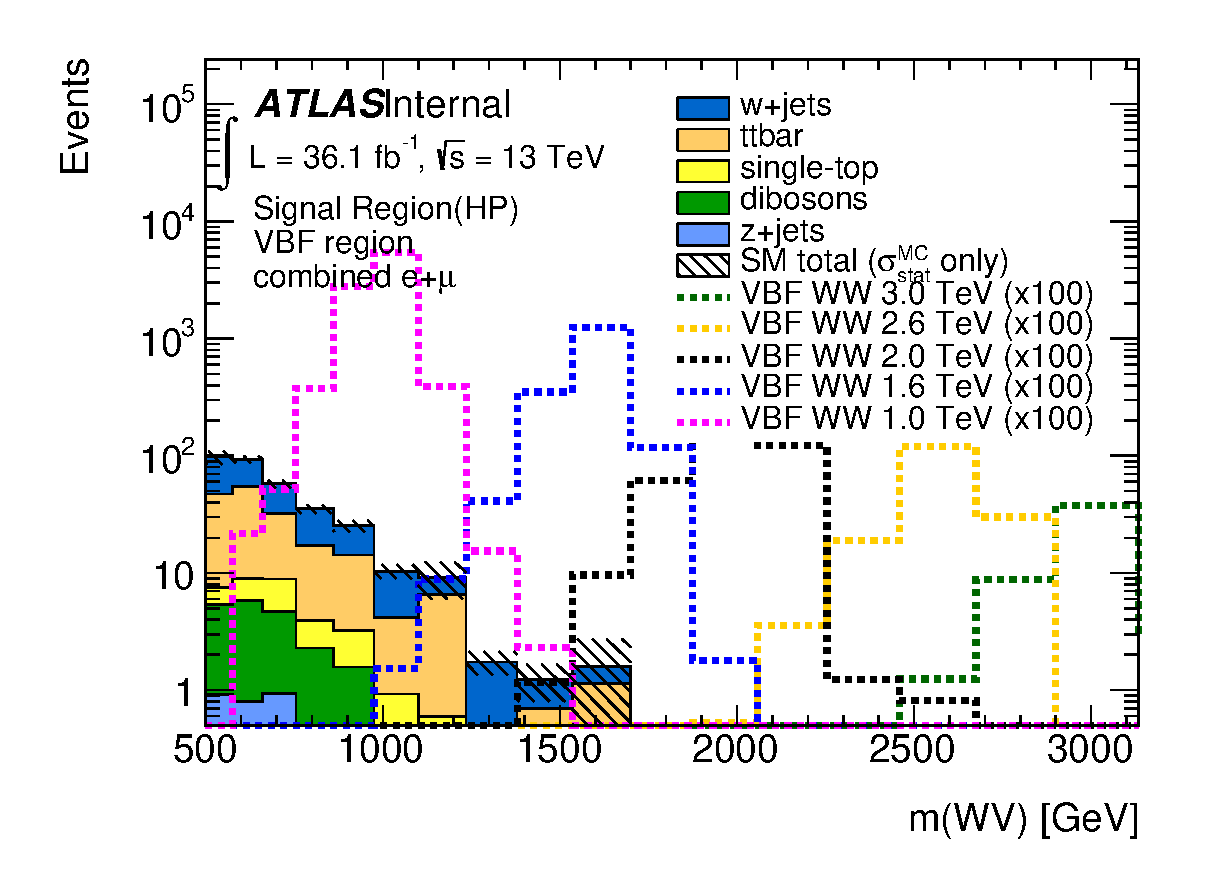
\includegraphics[width=.49\textwidth]{figures/EventSelection/VVM_0_comb_VBF}\label{fig:sig_mvv:a}}
\subfloat[]{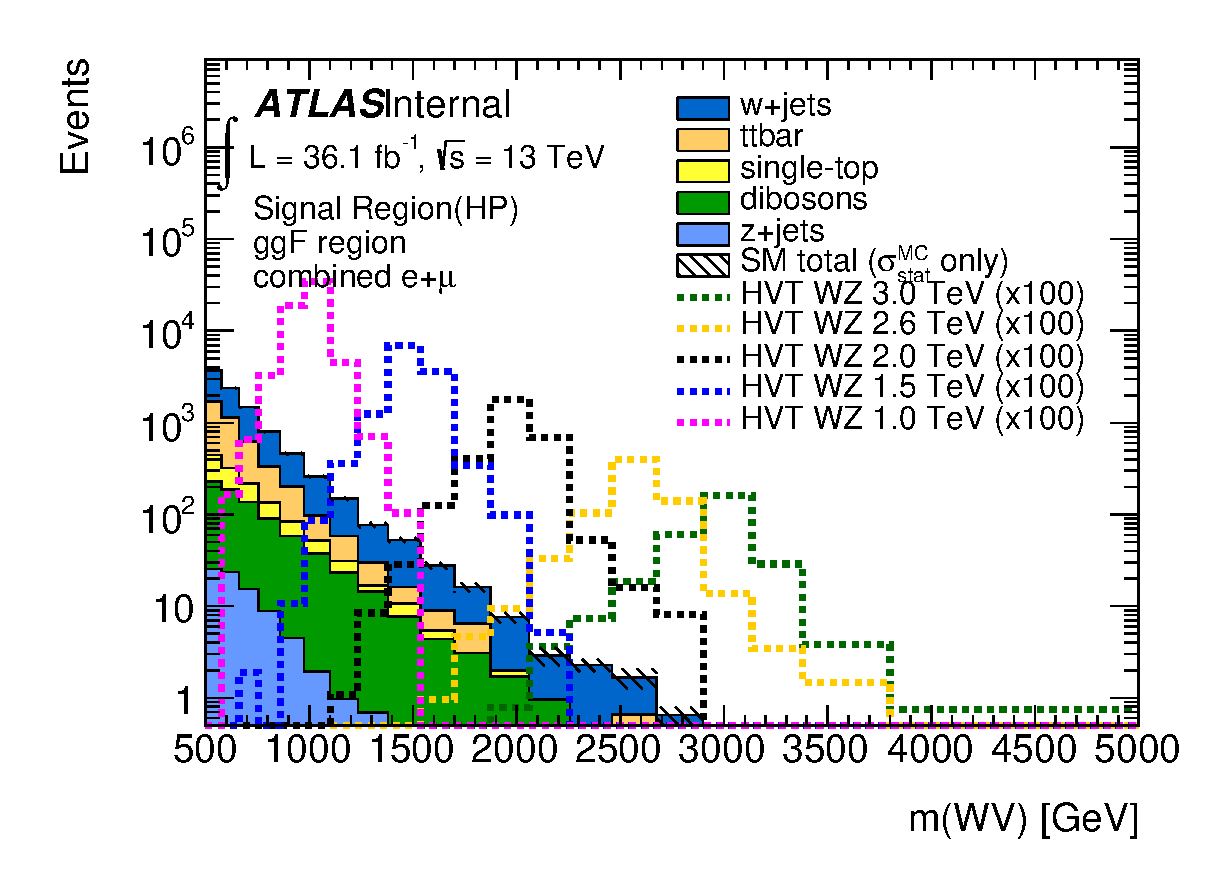
\includegraphics[width=.49\textwidth]{figures/EventSelection/VVM_0_comb_ggF}\label{fig:sig_mvv:b}}\\
\subfloat[]{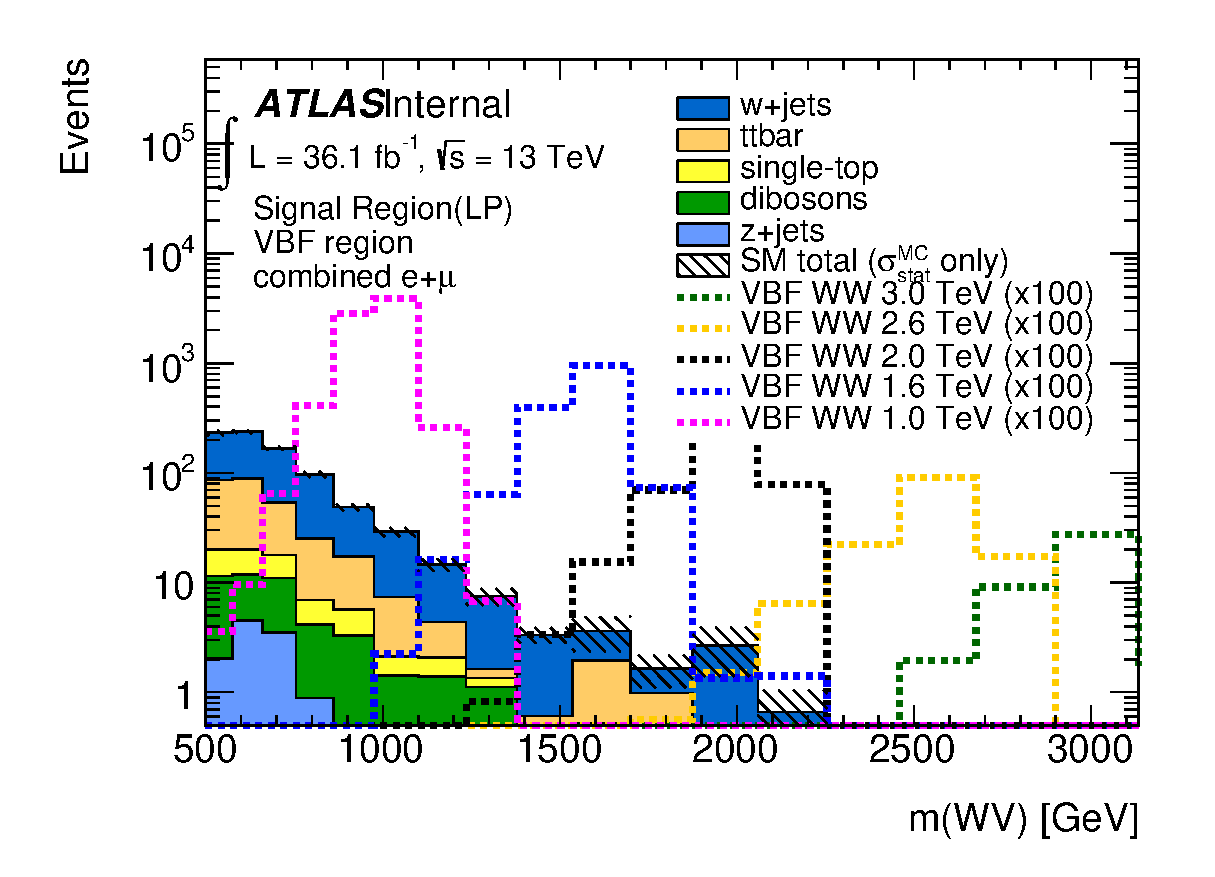
\includegraphics[width=.49\textwidth]{figures/EventSelection/VVM_11_comb_VBF}\label{fig:sig_mvv:c}}
\subfloat[]{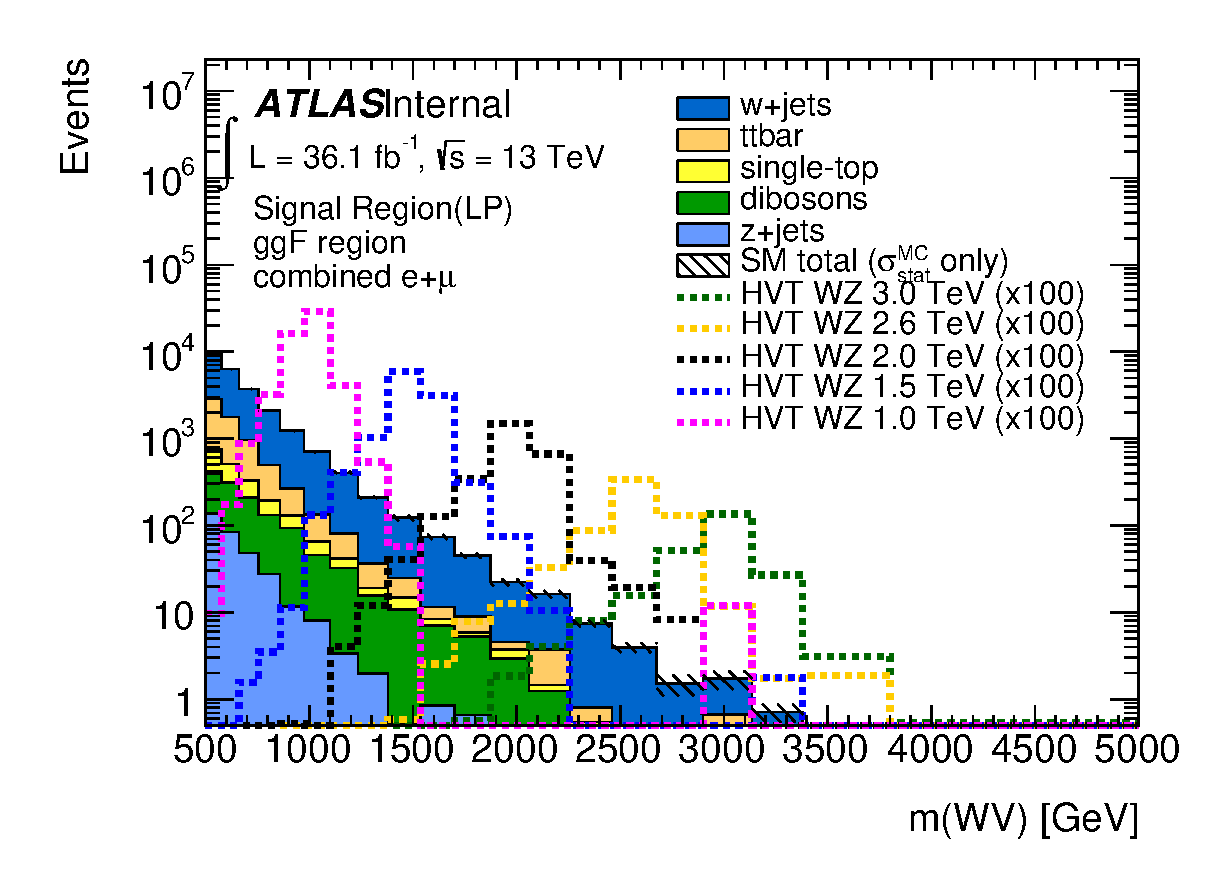
\includegraphics[width=.49\textwidth]{figures/EventSelection/VVM_11_comb_ggF}\label{fig:sig_mvv:d}}
\caption[Invariant mass distribution of signal and background samples in the signal regions]{The distribution of $m(WV\ra\ell\nu J)$ for simulated background and signal MC events, in the HP SR for \protect\subref{fig:sig_mvv:a} VBF selection and \protect\subref{fig:sig_mvv:b} ggF selection; and in the LP SR for \protect\subref{fig:sig_mvv:c} VBF selection and \protect\subref{fig:sig_mvv:d} ggF selection. Signal samples for masses between 1\,\TeV\, and 3\,\TeV\, are overlaid and scaled to 100 times the cross section. A scalar Higgs (HVT $W'$) model is used for the VBF (ggF) selection. All samples are scaled to an integrated luminosity of 36.1\,\ifb.}
\label{fig:sig_mvv}
\end{figure}

\begin{figure}[t]
\centering
\caption[Illustration of high purity and low purity signal region for large-R jets]{Illustration of $WW$ (shaded) and $WZ$ (dashed) HP and LP SRs for large-R jets. The SmoothedWZTagger 50\,\% and 80\,\% efficiency $V$-tagging working points define the HP (red) and LP (purple) regions. The value of the $D_2^{\beta=1}$ and mass window cuts depend on $\pt(J)$. The LP SR excludes the HP SR to ensure orthogonality. The $W+$jets CR is defined by the SR mass sidebands (orthogonal to both $WW$ and $WZ$ SR).}
\includegraphics[width=.75\textwidth]{figures/EventSelection/HPLPdefinition}
\label{fig:hplp_def}
\end{figure}
\begin{table}[b]
\centering
\begin{tabular}{l|l|c|c|c}
\hline\hline
\multicolumn{2}{l|}{Selection: HP (LP)} &SR&$W$ CR&\ttbar CR\\ \hline
Production& VBF & \multicolumn{3}{c}{ $m^{\textrm{VBF}}(j,j)>770\,\GeV$ and $|\Delta\eta^{\textrm{VBF}}(j,j)|>4.7$} \\ \cline{2-5}
Category& ggF & \multicolumn{3}{c}{Fail VBF selection} \\ \hline
&\vphantom{\Large B} Signal leptons & \multicolumn{3}{c}{ $1$} \\\cline{2-5}
&\vphantom{\Large B} Veto leptons & \multicolumn{3}{c}{ $0$} \\\cline{2-5}
$W\rightarrow \ell\nu$&\vphantom{\Large B} \met [\GeV]& \multicolumn{3}{c}{ $>100$ } \\ \cline{2-5}
%&\vphantom{\Large B} $\pt(\ell\nu)$ [\GeV]& \multicolumn{3}{c}{ $>200$ } \\ \cline{2-5}
&\vphantom{\Large B} $\met/\pt(e\nu) $ & \multicolumn{3}{c}{ $ > 0.2$ } \\\cline{2-5} 
&\vphantom{\Large B} $\pt(\ell\nu)$ [\GeV]& \multicolumn{3}{c}{ $>200$} \\\hline
&\vphantom{\Large B} Large-$R$ jets & \multicolumn{3}{c}{ $\geq 1$ } \\ \cline{2-5}
&\vphantom{\Large B} $D^{(\beta=1)}_2$ 50\,\% WP &pass (fail$\dagger$)&pass (fail)&pass (fail$\dagger$)\\ \cline{2-5}
$W/Z\rightarrow J$&\vphantom{\Large B} $D^{(\beta=1)}_2$ 80\,\% WP &--- (pass)&--- (pass)&--- (pass)\\ \cline{2-5}
&\vphantom{\Large B} $W/Z$ mass 50\,\% WP &pass (fail$\dagger$)&---  (---)&pass (fail$\dagger$)\\ \cline{2-5}
&\vphantom{\Large B} $W/Z$ mass 80\,\% WP &--- (pass)&fail (fail)&--- (pass)\\ \hline
Topology&\vphantom{\Large B} $\pt(\ell\nu) / m(WV)$ & \multicolumn{3}{c}{ $>0.3$ for VBF and $> 0.4$ for ggF selection}\\\cline{2-5}
Cuts&\vphantom{\Large B} $\pt(J) / m(WV)$ & \multicolumn{3}{c}{$>0.3$ for VBF and $> 0.4$ for ggF selection} \\ \hline
Num. $b$-jets&\vphantom{\Large B} $\Delta R(J,b)>1.0$ & \multicolumn{2}{c|}{0} &$\geq 1$ \\ \hline\hline
\end{tabular}
\caption[Event selection criteria]{Summary of the selection criteria used to define the SR, $W$+jets CR and \ttbar CR, for the HP and LP selections. The LP selections are listed in parentheses. Events are categorized according to their production mechanism where the VBF selection is prioritized.\\ $\dagger$ For the LP SR and LP \ttbar CR, the large-R jet can fail either the 50\,\% efficiency $D_2^{\beta=1}$ working point or the 50\,\% efficiency mass window working point. } 
\label{tab:SRdefinitions}
\end{table}
%\end{figure}

%
\clearpage
\section{Signal Efficiency and Acceptance}
\label{ch:evt_sel:sig_eff}
Signal efficiency times acceptance ($\epsilon\times A$) is defined as the ratio of the number of reconstructed signal events passing the signal region selection, to the total number of generated signal events. In~\Fig{\ref{fig:sig_acc_vbf}} and~\Fig{\ref{fig:sig_acc_ggf}}, $\epsilon\times A$ is plotted as a function of $m(WV\ra\ell\nu J)$ for all signal models with VBF production and ggF (or qqF) production, respectively. \Fig{\ref{fig:sig_acc_vbf}} shows that, for signal models with VBF production, a substantial fraction of signal events leak into the ggF selection category, and the overall $\epsilon\times A$ is smaller than for samples with ggF (or qqF) production. Less than 1\,\% of signals produced by ggF (or qqF) leak into the VBF selection category. Due to these factors, and the smaller cross section for models with VBF production, the VBF selection is prioritized over the ggF selection to increase the sensitivity of the search.

The search is most efficient for higher resonance masses, with most signal models reaching a plateau in $\epsilon\times A$ for $m(WV)>1\,\TeV$. For the models with ggF (or qqF) production, the plateau region corresponds to a total $\epsilon\times A$ between approximately 30\,\% and 35\,\%. The scalar heavy Higgs samples notably have a smaller total $\epsilon\times A$, approximately 20\,\% to 23\,\%. 
In models of higher spin resonances, the two weak bosons are preferentially produced in the central barrel region, while in the scalar resonance model, the production angle of the two weak bosons is uniformly distributed.
%The distribution of the two weak bosons is more peaked in the central barrel region for higher spin resonances than in scalar resonance models. 
Thus, the cuts on $\pT(V)/m(WV)$ reject more signal events for the scalar resonance model than for higher spin resonance models, since a larger fraction of the daughter weak bosons will be produced at larger $|\eta|$, with correspondingly lower \pT, in the scalar model. For most mass points, there is approximately a 50\,\% increase in $\epsilon\times A$ by including the LP SR in addition to the HP SR.

\begin{figure}[tbp]
\centering
\subfloat[]{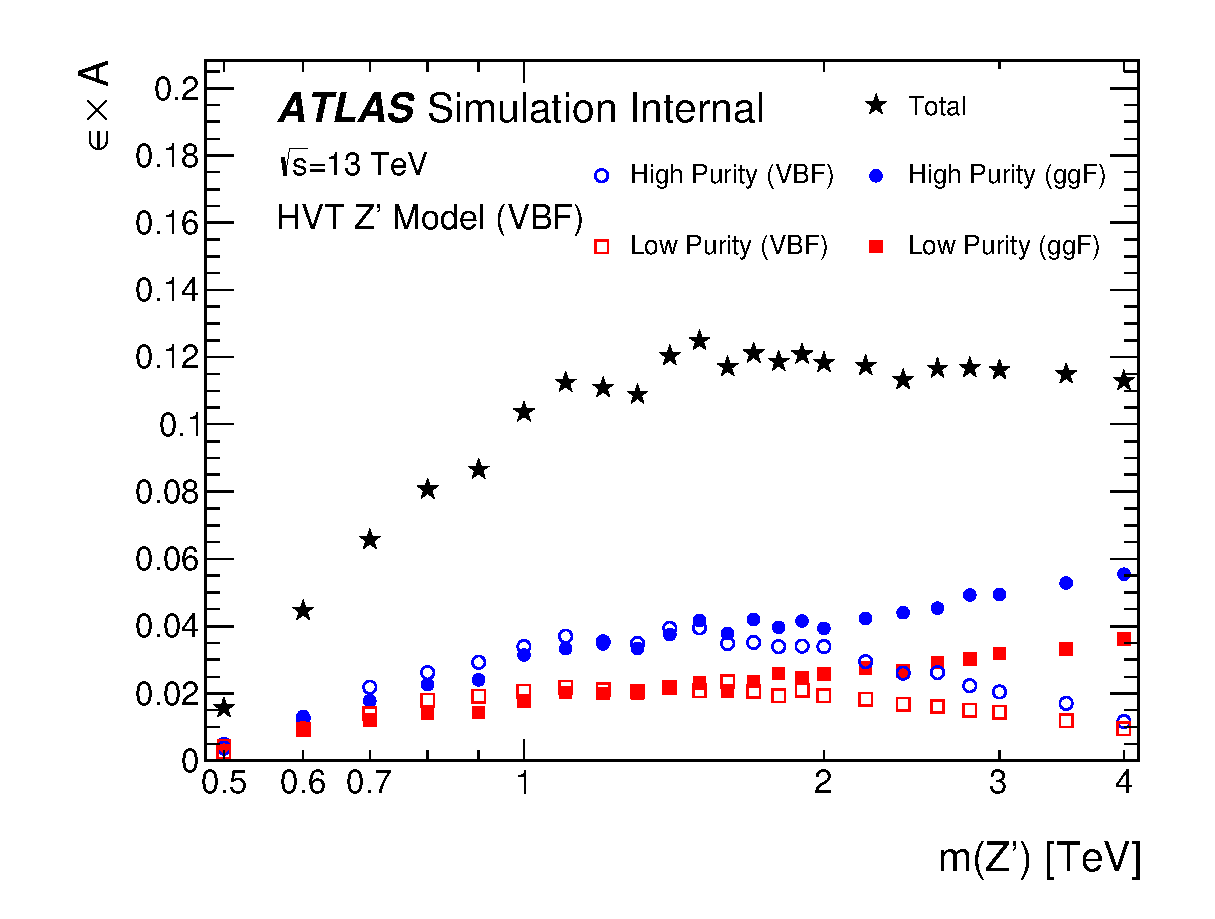
\includegraphics[width=.49\textwidth]{figures/EventSelection/VBF-HVTWW_effacc}\label{fig:sig_acc_vbf:a}}
\subfloat[]{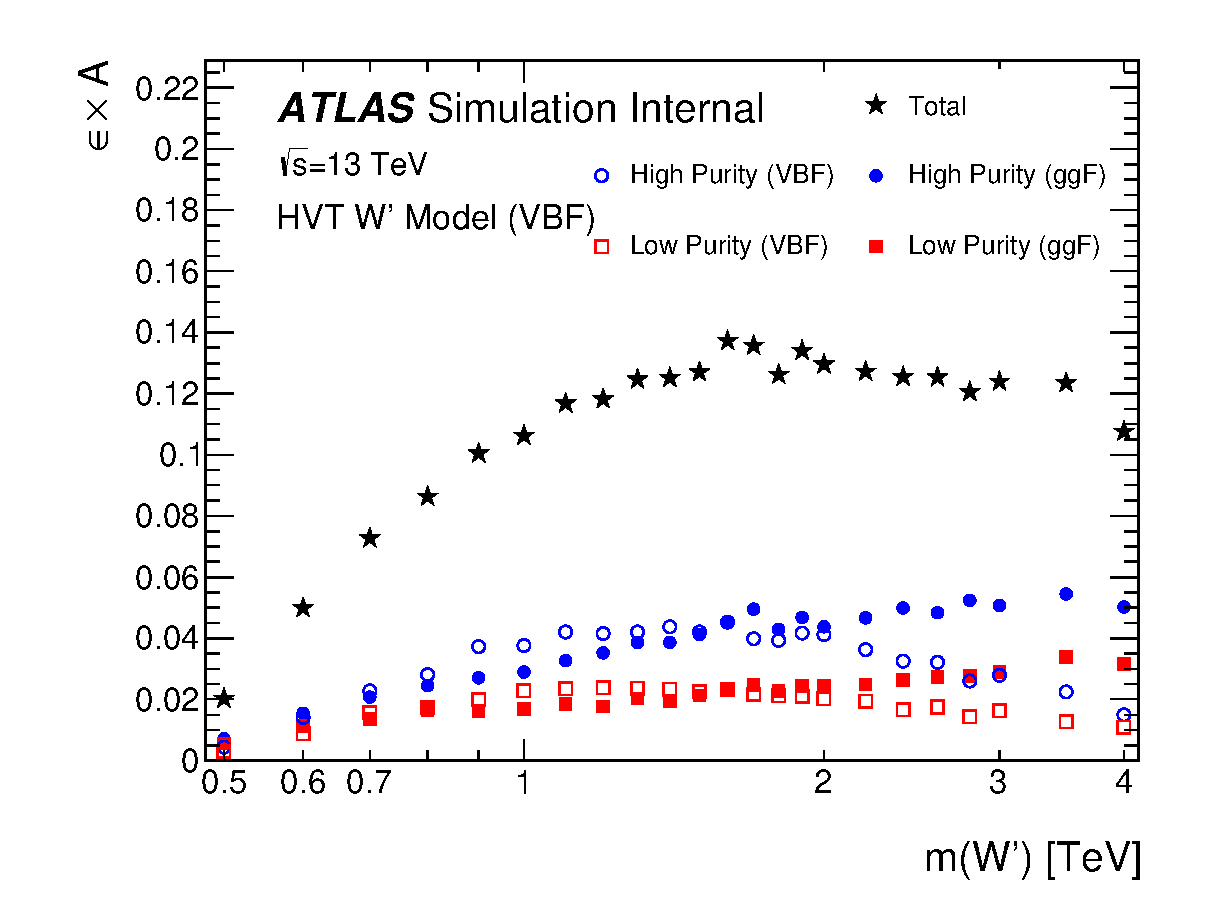
\includegraphics[width=.49\textwidth]{figures/EventSelection/VBF-HVTWZ_effacc}\label{fig:sig_acc_vbf:b}}\\
\subfloat[]{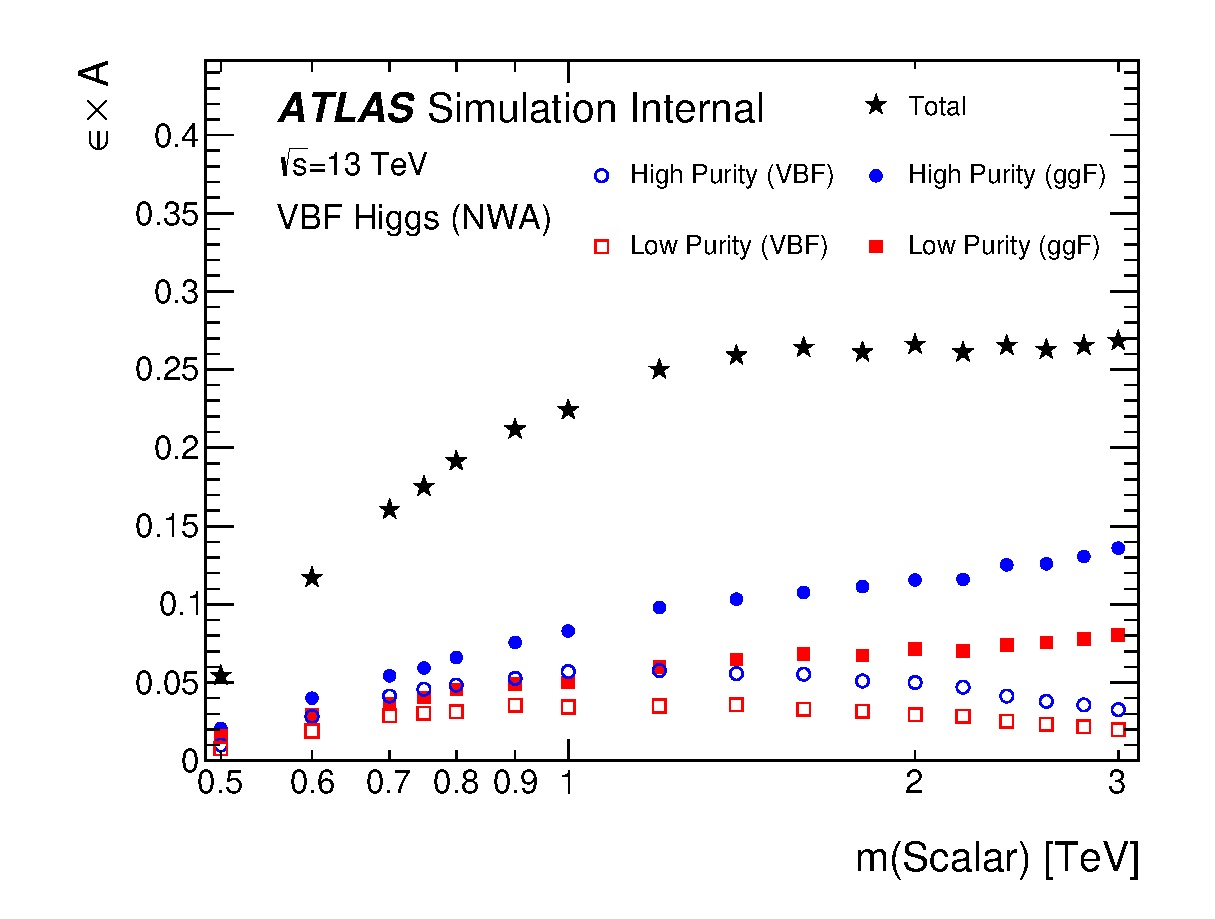
\includegraphics[width=.49\textwidth]{figures/EventSelection/VBFWWNWA_effacc}\label{fig:sig_acc_vbf:c}}
\caption[Signal efficiency times acceptance for models with vector boson fusion production]{Signal efficiency times acceptance ($\epsilon\times A$) is plotted as a function of $m(WV\ra\ell\nu J)$ for models with VBF production in the high purity (blue) and low purity (red) VBF selection (hollow) and ggF selection (filled) categories, as well as the total combined $\epsilon\times A$ (black star). The signal models include \protect\subref{fig:sig_acc_vbf:a} an HVT $Z'$, \protect\subref{fig:sig_acc_vbf:b} an HVT $W'$, and \protect\subref{fig:sig_acc_vbf:c} a scalar heavy Higgs (NWA). $\epsilon\times A$ is defined as the ratio of the number of signal events reconstructed in the signal region, to the total number of generated signal events. }
\label{fig:sig_acc_vbf}
\end{figure}

\begin{figure}[tbp]
\centering
\subfloat[]{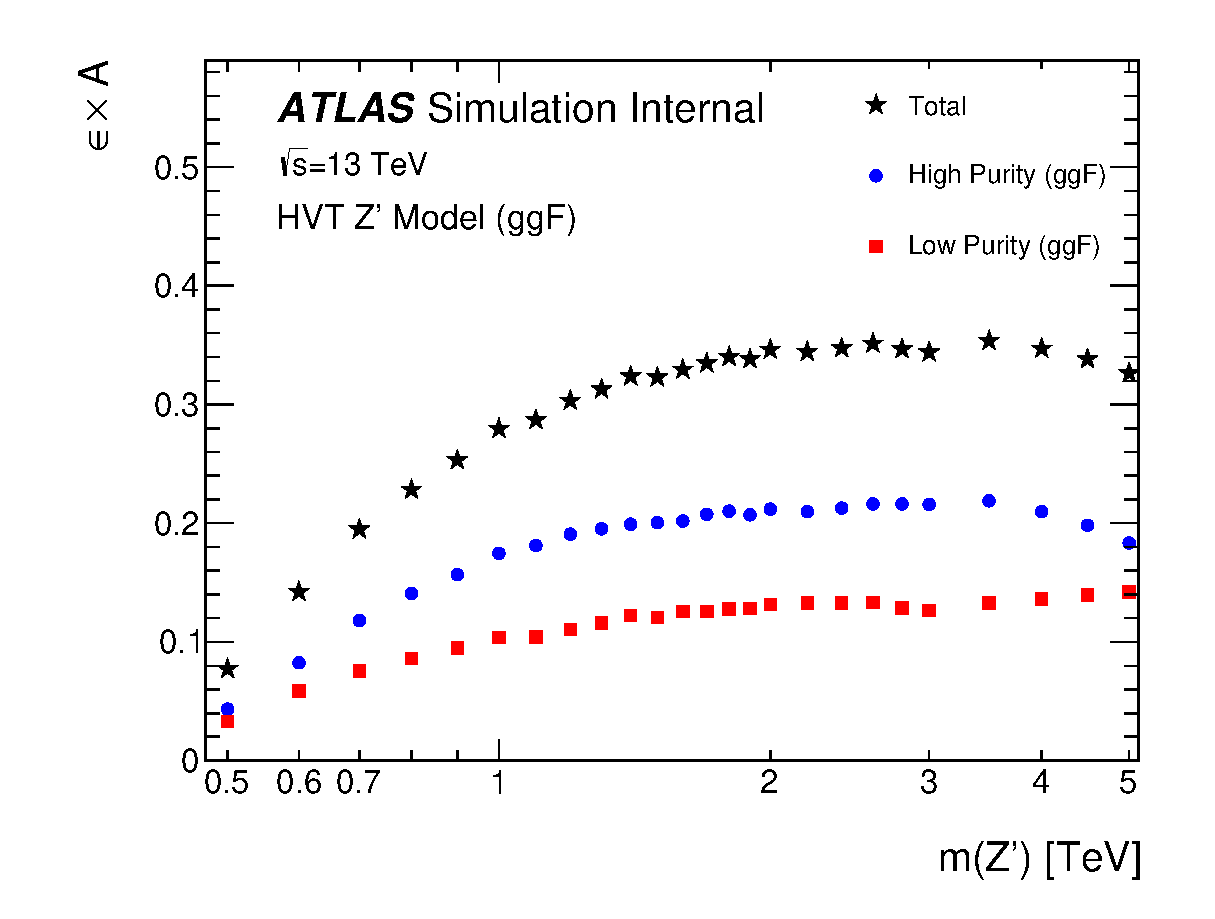
\includegraphics[width=.49\textwidth]{figures/EventSelection/HVTWW_effacc}\label{fig:sig_acc_ggf:a}}
\subfloat[]{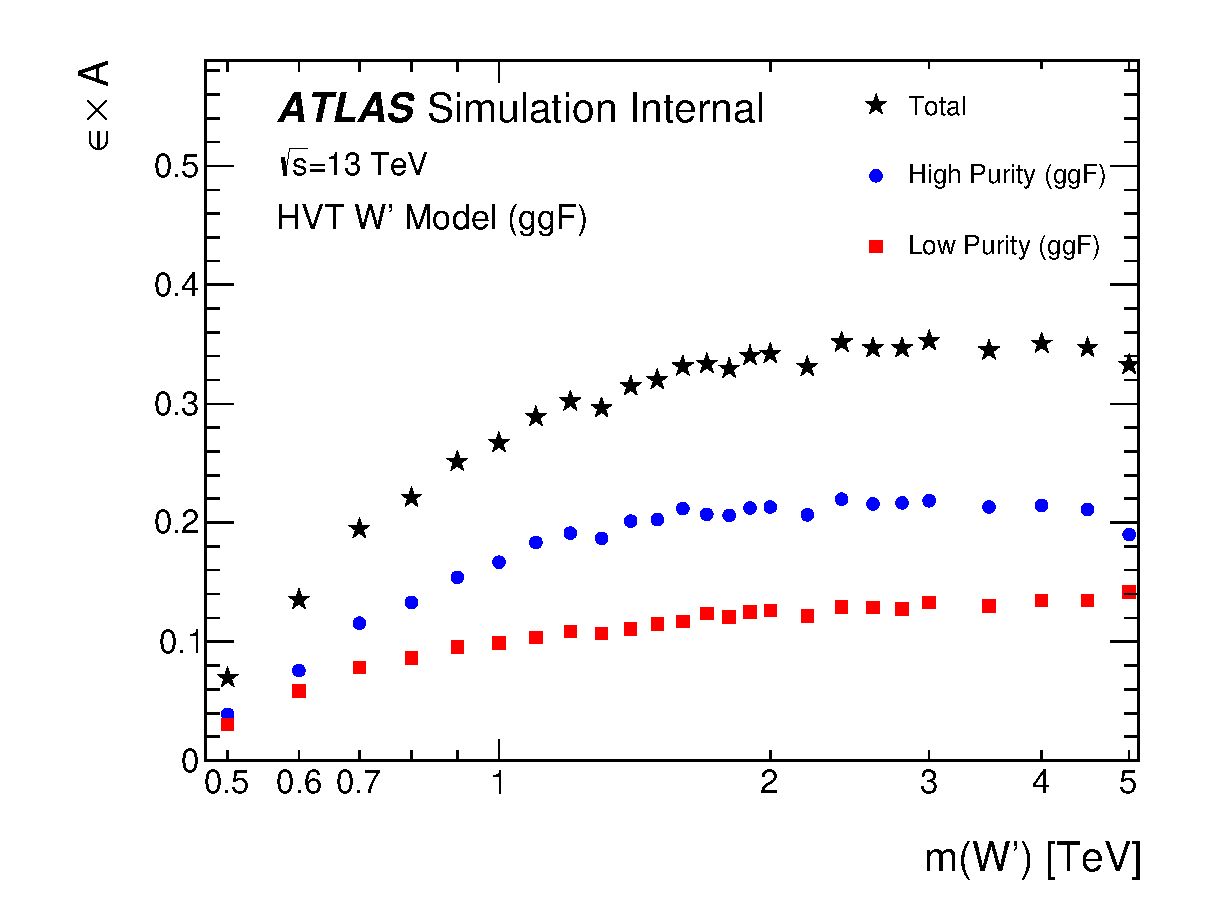
\includegraphics[width=.49\textwidth]{figures/EventSelection/HVTWZ_effacc}\label{fig:sig_acc_ggf:b}}\\
\subfloat[]{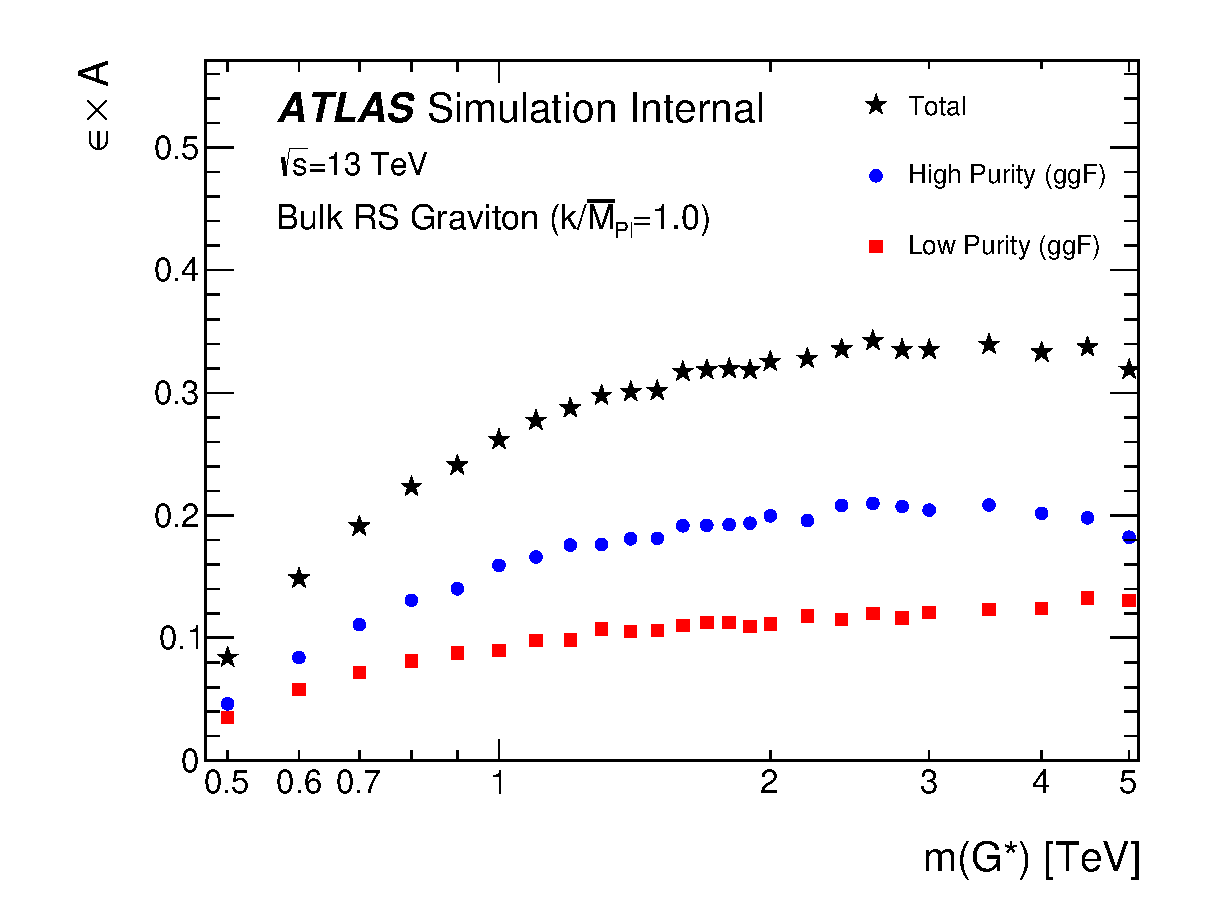
\includegraphics[width=.49\textwidth]{figures/EventSelection/RSGWW_effacc}\label{fig:sig_acc_ggf:c}}
\subfloat[]{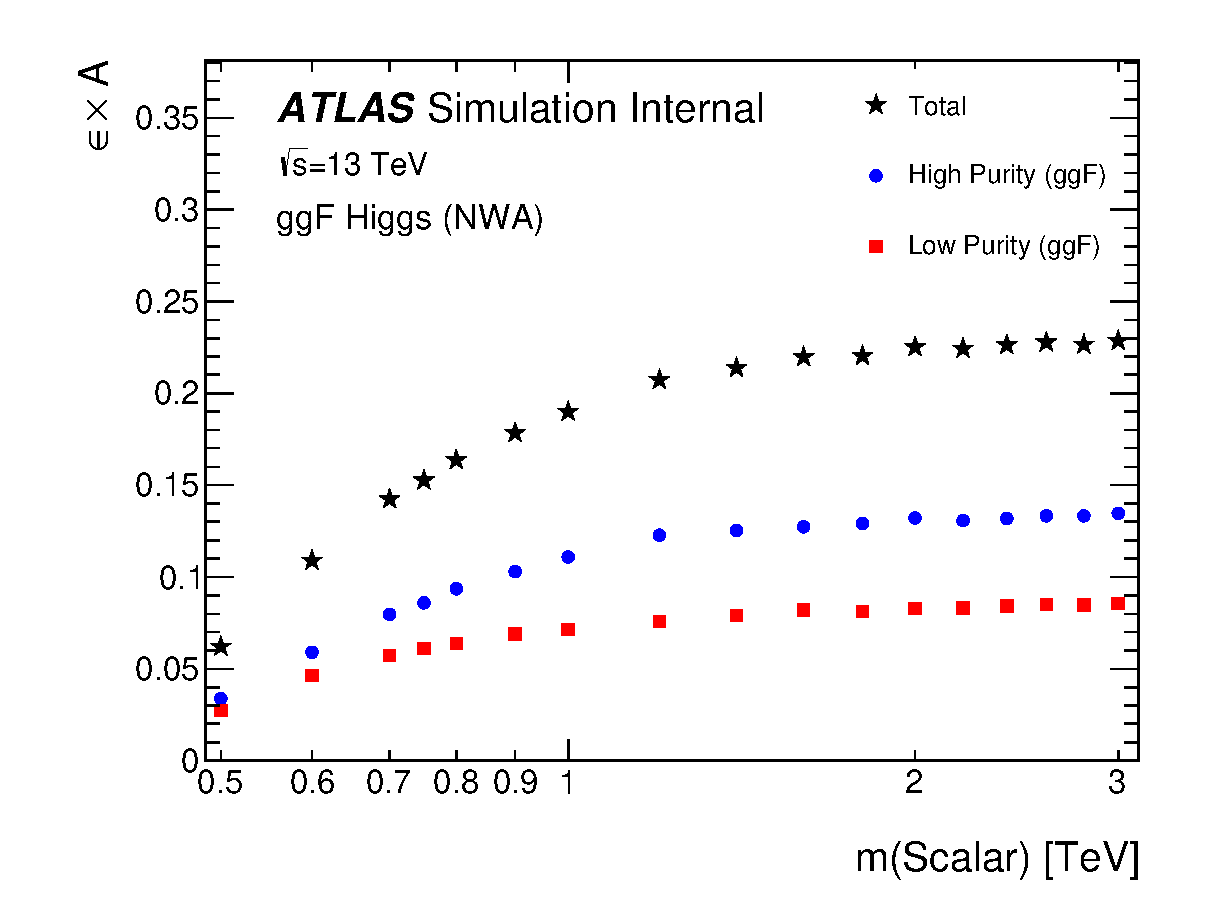
\includegraphics[width=.49\textwidth]{figures/EventSelection/ggHWWNWA_effacc}\label{fig:sig_acc_ggf:d}}
\caption[Signal efficiency times acceptance for models with gluon gluon fusion production]{Signal efficiency times acceptance ($\epsilon\times A$) is plotted as a function of $m(WV\ra\ell\nu J)$ for models with ggF (or qqF) production in the high purity (blue) and low purity (red) ggF selection categories, as well as the total combined $\epsilon\times A$ (black star). The signal models include \protect\subref{fig:sig_acc_ggf:a} an HVT $Z'$, \protect\subref{fig:sig_acc_ggf:b} an HVT $W'$, \protect\subref{fig:sig_acc_ggf:c} a bulk RS Graviton ($k/\overline{M}_{\textrm Pl}=1.0$), and \protect\subref{fig:sig_acc_ggf:d} a scalar heavy Higgs (NWA). $\epsilon\times A$ is defined as the ratio of the number of signal events reconstructed in the signal region, to the total number of generated signal events.}
\label{fig:sig_acc_ggf}
\end{figure}

%
\clearpage
\section{Background Validation}
To validate the background modeling in the control regions, recorded data is overlaid with the background predicted using MC samples. The $m(\ell\nu J)$ distribution is shown in the HP CRs in~\Fig{\ref{fig:datamc_hpcr}}, and in the LP CRs in~\Fig{\ref{fig:datamc_lpcr}}. The ratio of the data to the MC prediction is included, with MC statistical uncertainties overlaid. 

In most regions, the agreement is fairly good, with no noticeable slopes in the ratio plot. The MC samples in the \Wjets CRs predict a higher event yield than is observed. However, the overall normalization will be determined by the fit in~\Ch{\ref{ch:stats}}, and therefore it is only important to examine the agreement in the slopes of the distributions. The CRs for the VBF selection in general show a larger normalization discrepancy between data and MC prediction, with respect to the ggF selection. This behavior has been observed in other similar analyses at ATLAS, and is not an issue in this search because separate normalizations will be determined for the ggF and VBF selections. Distributions for all major kinematic variables related to the event selection were checked, and a similar level of agreement was observed. After the fit, systematic uncertainties (\Ch{\ref{ch:syst}}) will be included in the uncertainty bands, representing a more conservative total estimated uncertainty. 

\begin{figure}[htbp]
\centering
\subfloat[]{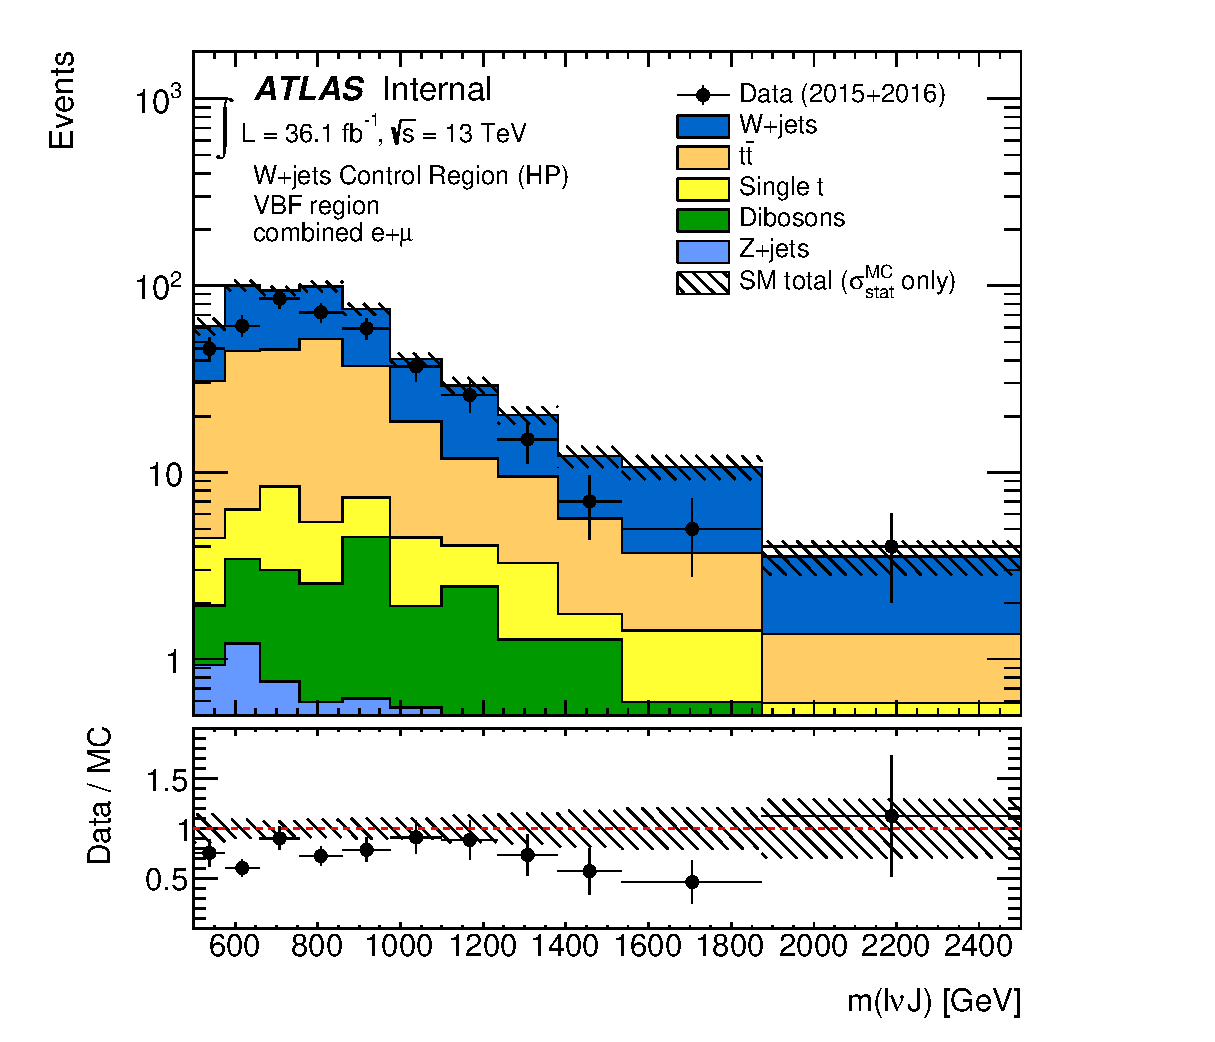
\includegraphics[width=.48\textwidth]{figures/BackgroundValidation/VVM_3_comb_VBF}\label{fig:datamc_hpcr:a}}
\subfloat[]{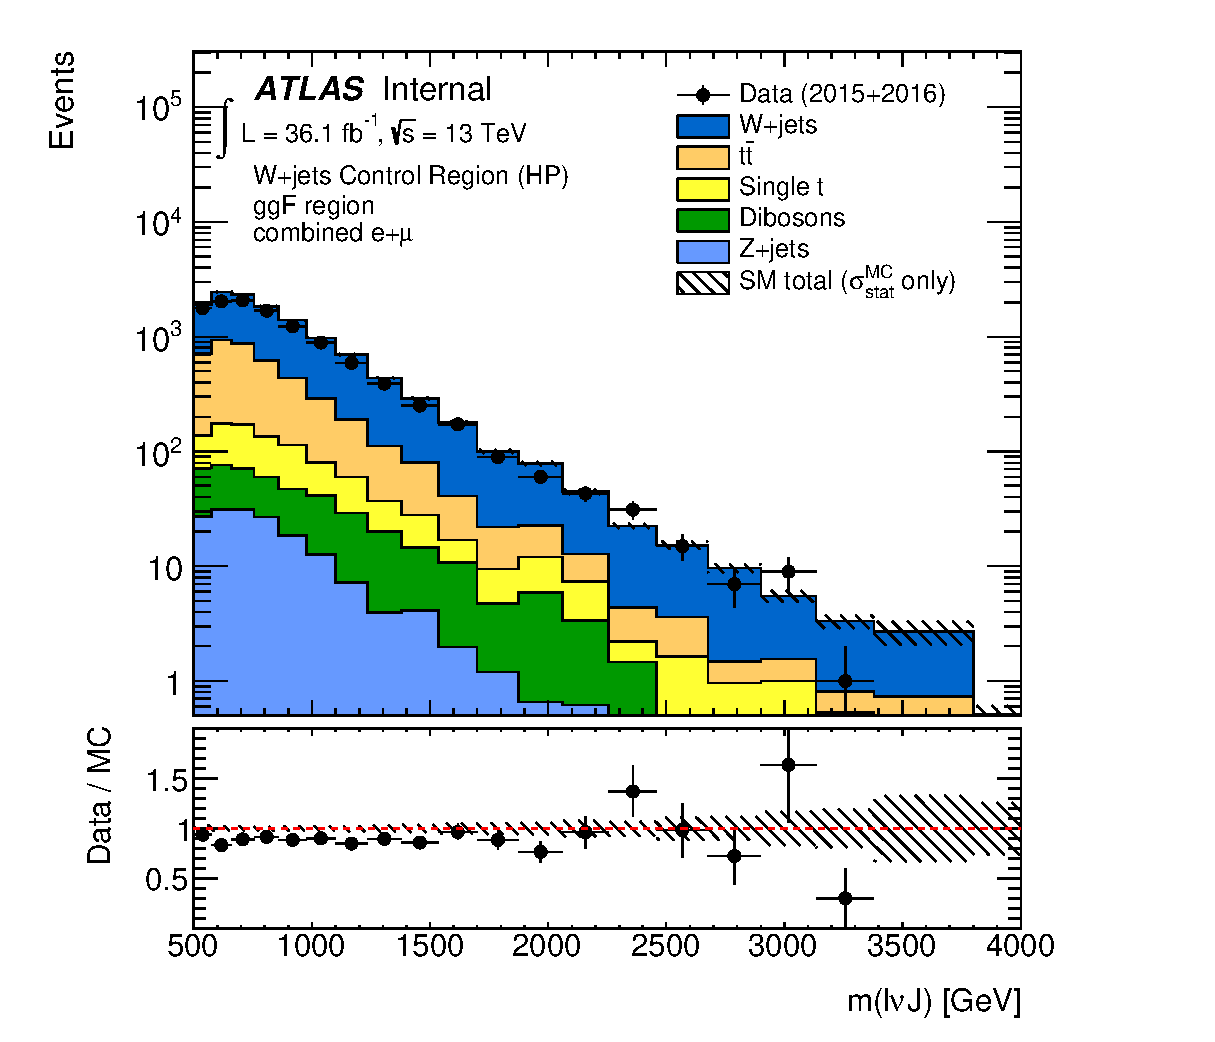
\includegraphics[width=.48\textwidth]{figures/BackgroundValidation/VVM_3_comb_ggF}\label{fig:datamc_hpcr:b}}\\
\subfloat[]{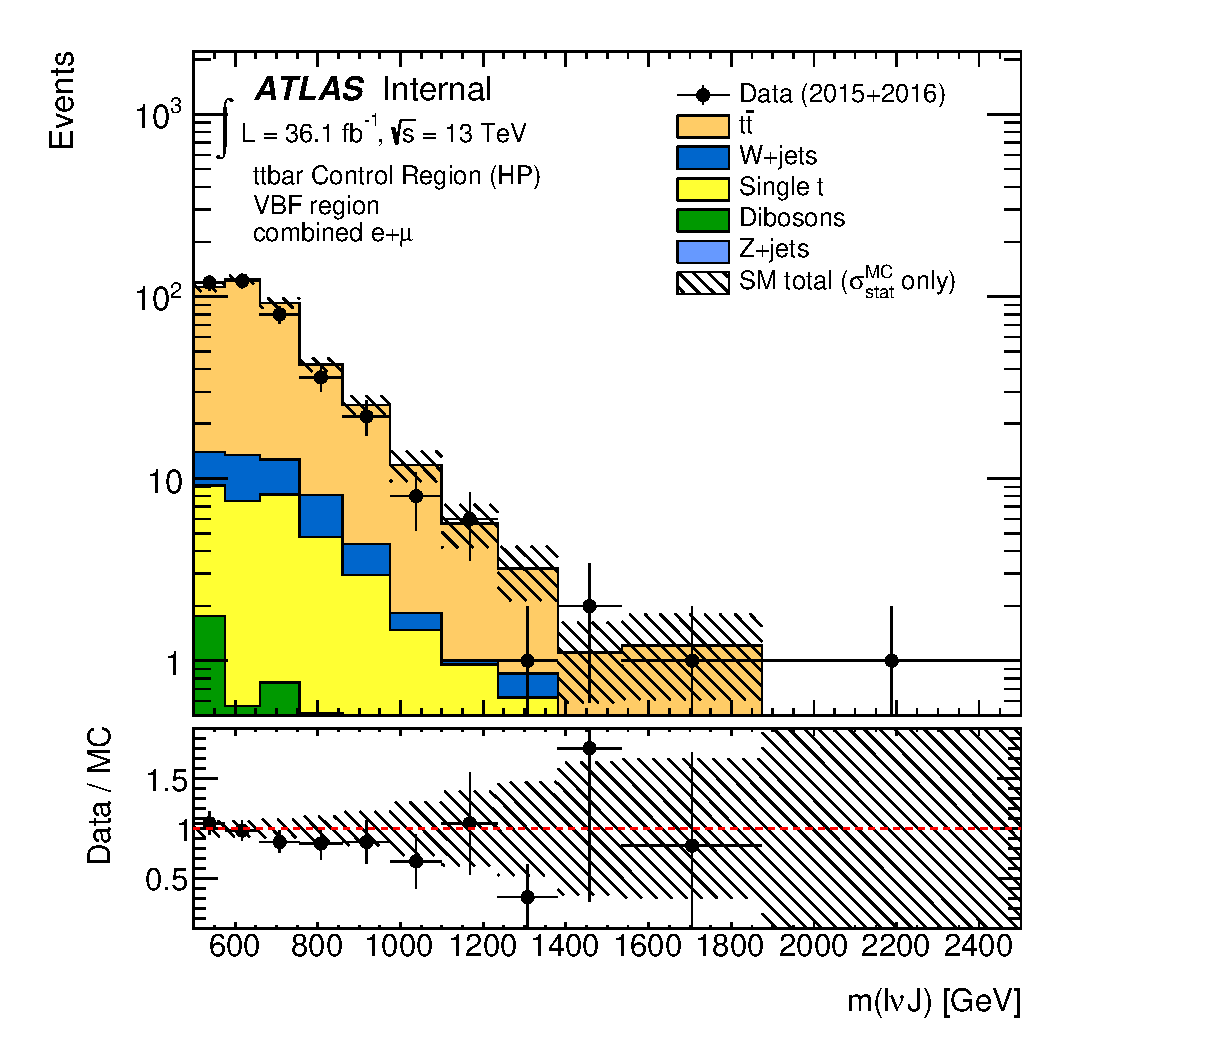
\includegraphics[width=.48\textwidth]{figures/BackgroundValidation/VVM_2_comb_VBF}\label{fig:datamc_hpcr:c}}
\subfloat[]{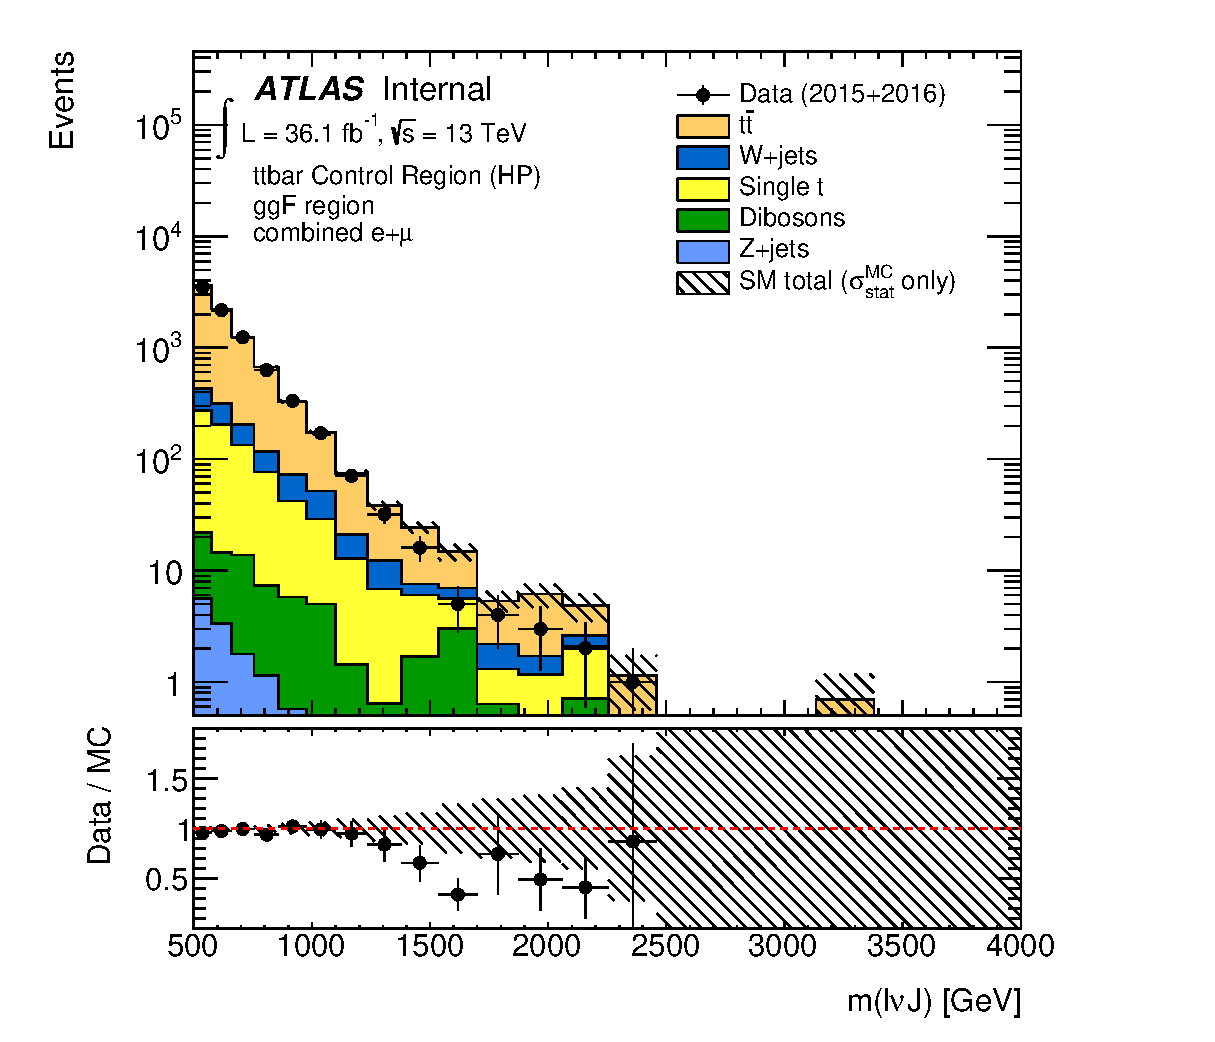
\includegraphics[width=.48\textwidth]{figures/BackgroundValidation/VVM_2_comb_ggF}\label{fig:datamc_hpcr:d}}
\caption[Data and Monte Carlo comparison in the high purity control regions]{The distribution of $m(\ell\nu J)$ for data from 2015+2016 (36.1\,\ifb) and for the background MC prediction. The VBF selection HP \protect\subref{fig:datamc_hpcr:a} \Wjets CR and \protect\subref{fig:datamc_hpcr:c} \ttbar CR, and the ggF selection HP \protect\subref{fig:datamc_hpcr:b} \Wjets CR and \protect\subref{fig:datamc_hpcr:d} \ttbar CR, are shown. The simulated MC backgrounds are normalized to the recorded luminosity. In the bottom panel, the ratio of the observed data to MC prediction is plotted, with the MC statistical uncertainty overlaid as the shaded band. }
\label{fig:datamc_hpcr}
\end{figure}

\begin{figure}[htbp]
\centering
\subfloat[]{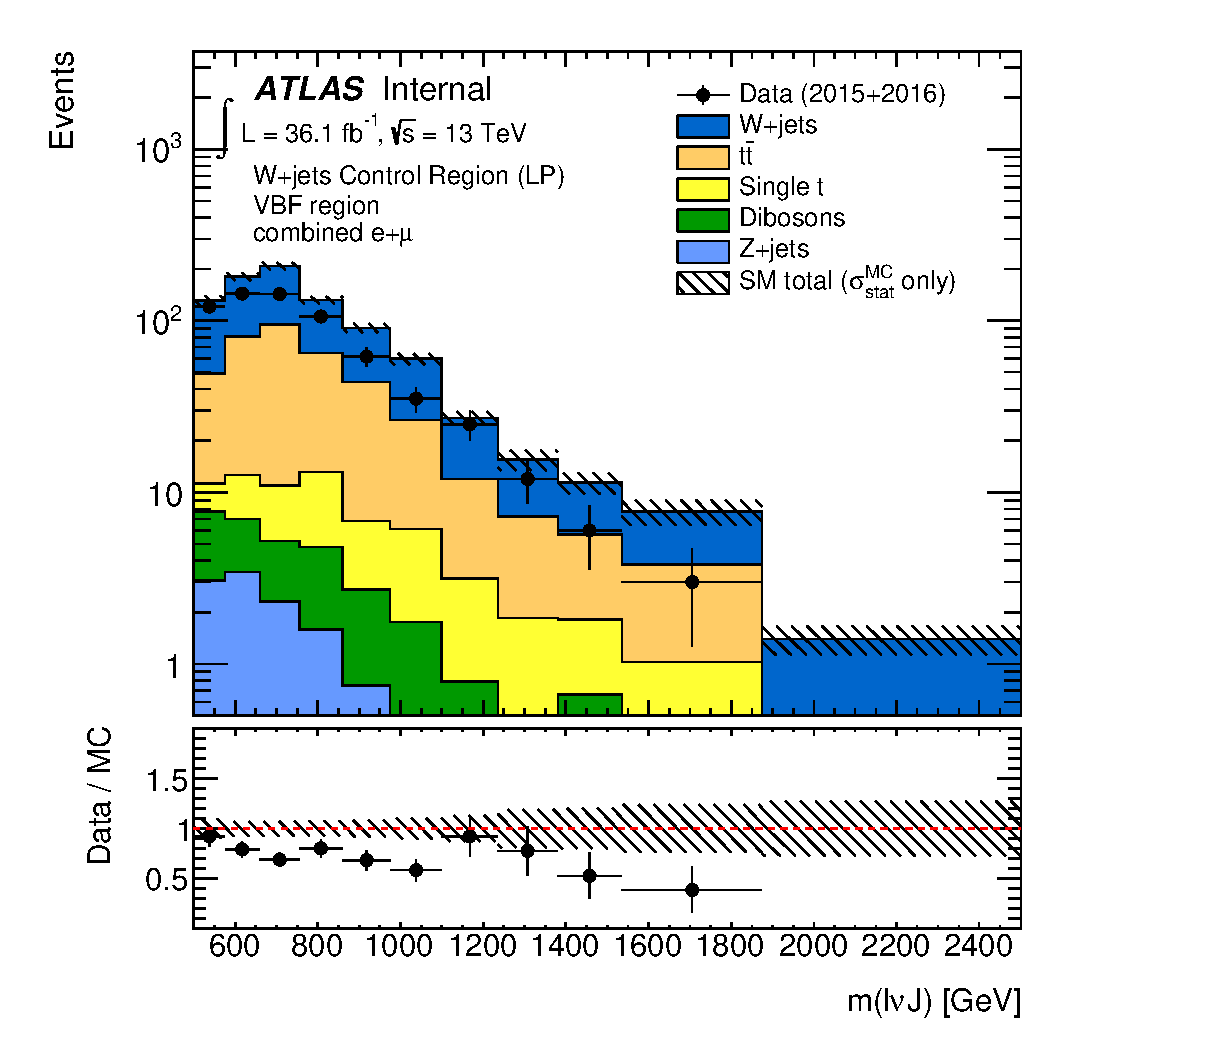
\includegraphics[width=.48\textwidth]{figures/BackgroundValidation/VVM_12_comb_VBF}\label{fig:datamc_lpcr:a}}
\subfloat[]{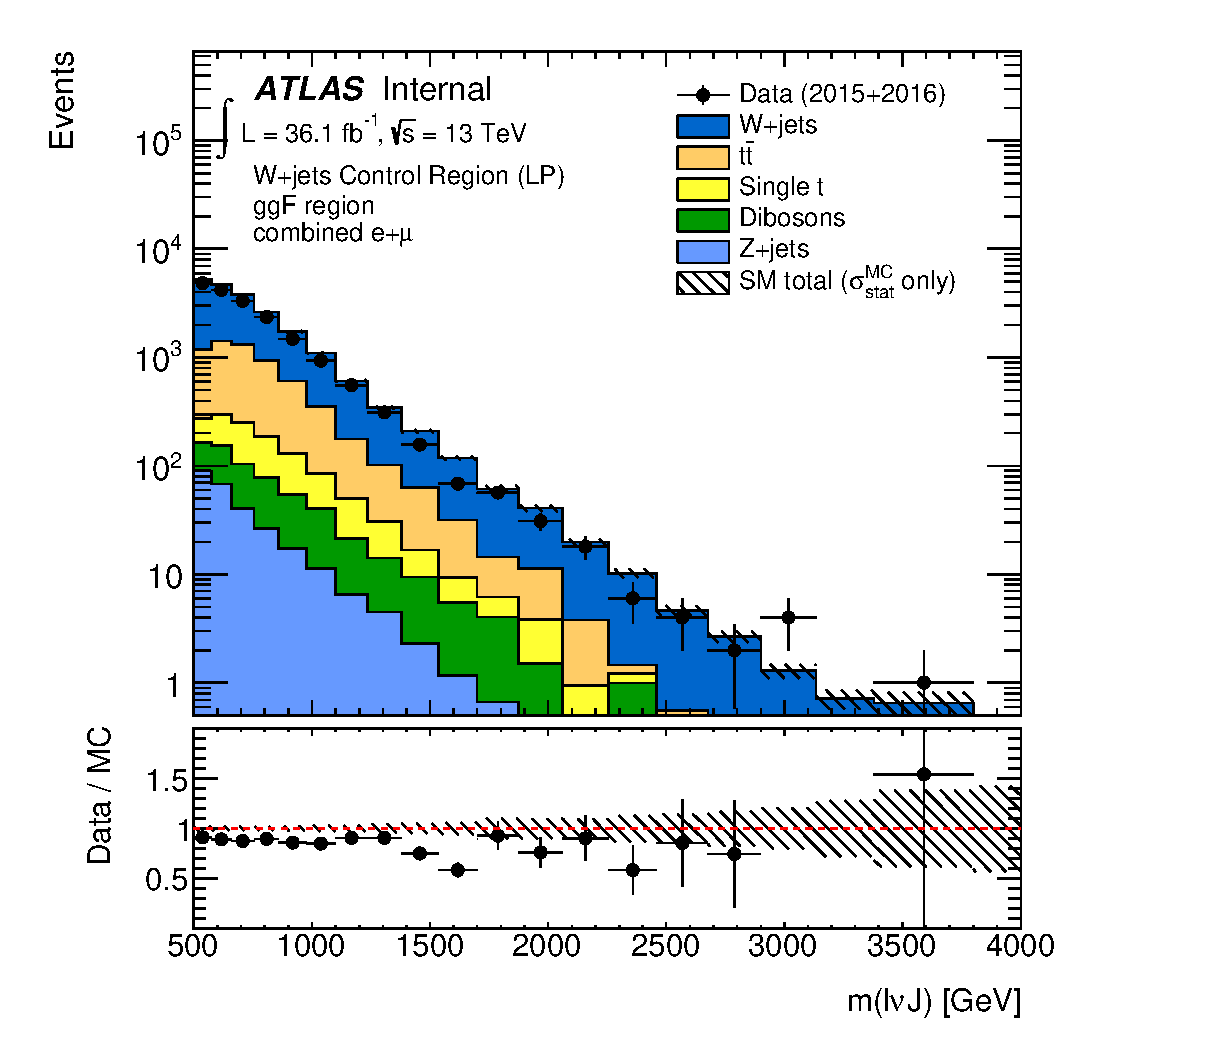
\includegraphics[width=.48\textwidth]{figures/BackgroundValidation/VVM_12_comb_ggF}\label{fig:datamc_lpcr:b}}\\
\subfloat[]{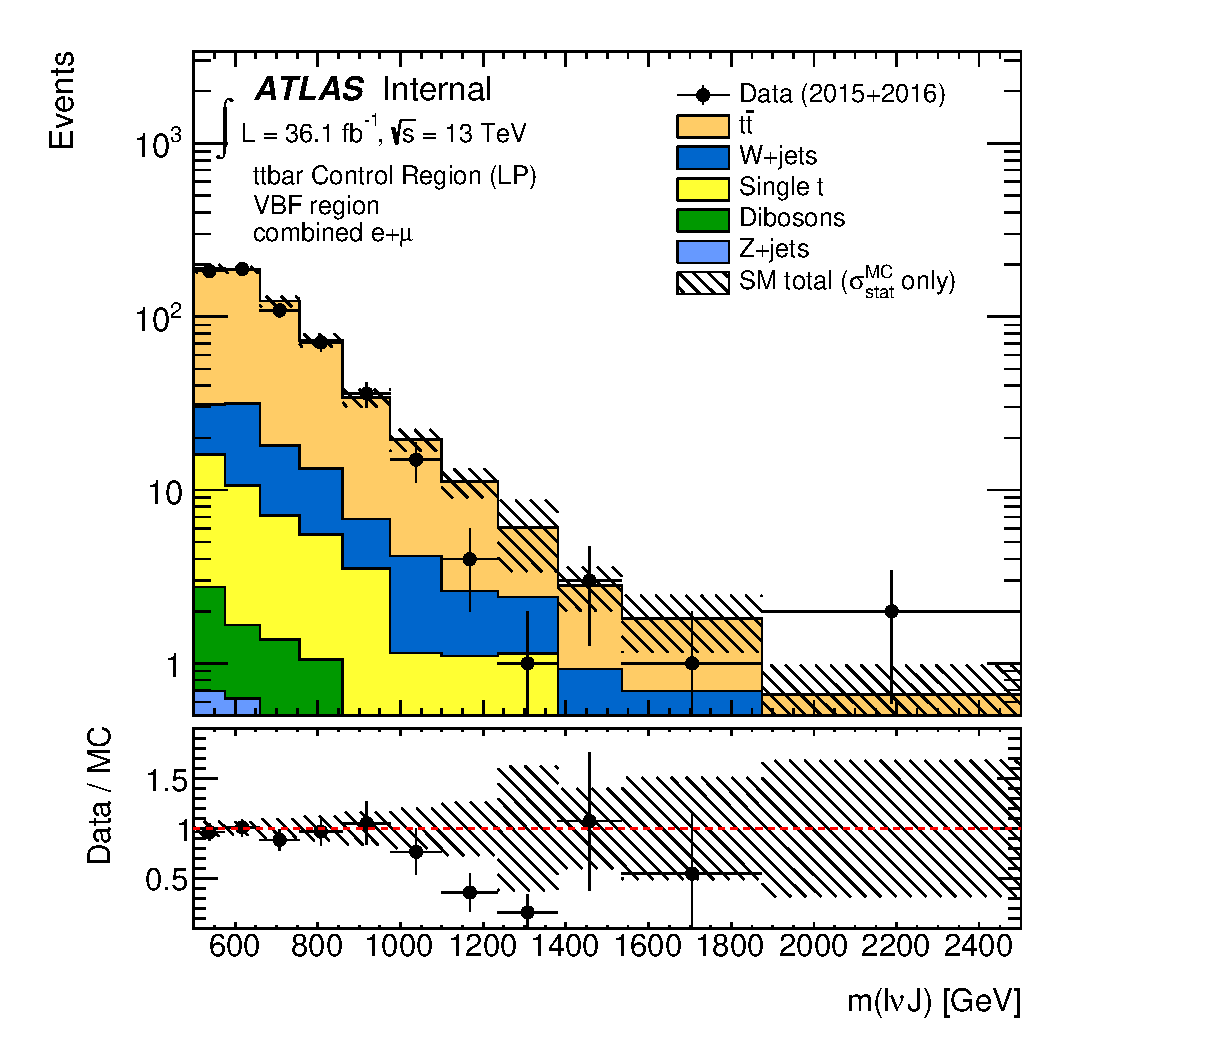
\includegraphics[width=.48\textwidth]{figures/BackgroundValidation/VVM_13_comb_VBF}\label{fig:datamc_lpcr:c}}
\subfloat[]{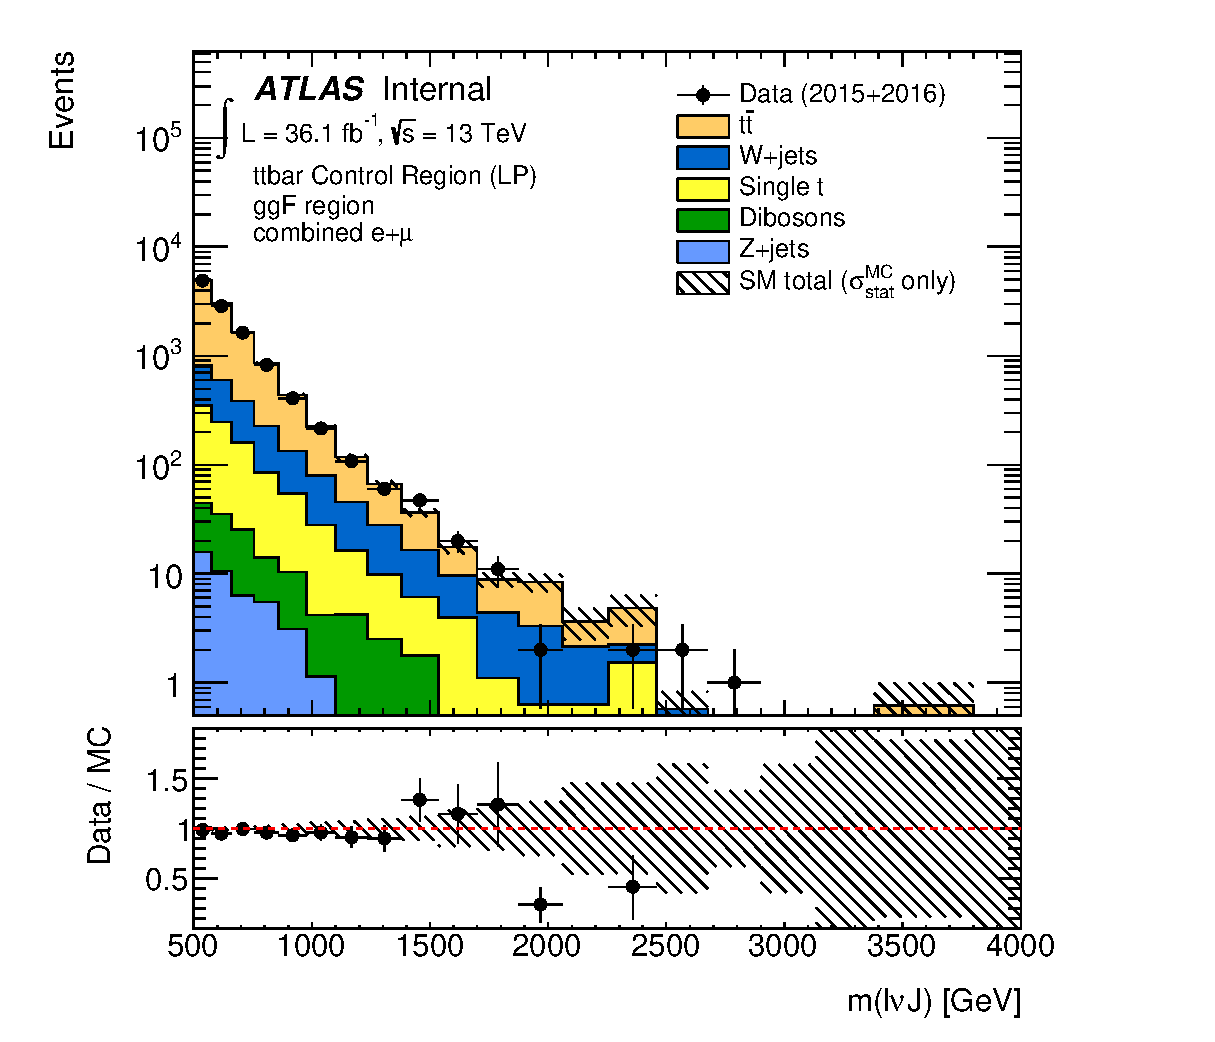
\includegraphics[width=.48\textwidth]{figures/BackgroundValidation/VVM_13_comb_ggF}\label{fig:datamc_lpcr:d}}
\caption[Data and Monte Carlo comparison in the low purity control regions]{The distribution of $m(\ell\nu J)$ for data from 2015+2016 (36.1\,\ifb) and for background MC prediction. The VBF selection LP \protect\subref{fig:datamc_lpcr:a} \Wjets CR and \protect\subref{fig:datamc_lpcr:c} \ttbar CR, and ggF selection LP \protect\subref{fig:datamc_lpcr:b} \Wjets CR and \protect\subref{fig:datamc_lpcr:d} \ttbar CR, are shown. The simulated MC backgrounds are normalized to the recorded luminosity. In the bottom panel, the ratio of the observed data to MC prediction is plotted, with the MC statistical uncertainty overlaid as the shaded band.}
\label{fig:datamc_lpcr}
\end{figure}


